\chapter{Информационное взаимодействие компонентов модульного технологического оборудования}\label{ch:ch3}

\section{Подсистема управления модульным оборудованием}\label{sec:ch3/sec1}

Современные системы управления технологическим оборудованием сложны и надежны. Каждый их элемент представляет собой черный ящик с жесткой иерархической архитектурой. Все в таких системах ориентировано на обеспечение качества, надежности и отказоустойчивости. Инерциальность в развитии таких систем вынуждает разработчиков использовать монолитную архитектуру, поскольку оборудование с распределенным управлением не может быть легко добавлено в распределенную производственную среду.

Следовательно, акцент делается на интеграции. Другими словами, разработчики сосредоточились на объединении разнородных компонентов в одну производственную систему вместо использования концепции взаимодействия (интероперабельности). Концепция взаимодействия влечет за собой создание открытого интерфейса, который позволяет компонентам оставаться в автономном состоянии с возможностью обмена данными.

Рассматриваемое модульное оборудование требует переосмысления данного подхода и создания системы управления, которая состоит из взаимозаменяемых <<строительных блоков>> с описанной унификацией ввода и вывода. При создании новой конфигурации оборудования (установке модуля/модулей на шасси) должна автоматически изменяться и подсистема управления получившимся оборудованием. Следовательно, устройство ЧПУ должно знать о каждом возможном модуле заранее, то есть снова будет получена монолитная система с иерархическим управлением.

Таким образом, необходимо выделить основную часть архитектуры и определить спецификации в отношении протокола связи, а также правила создания новых программных и аппаратных модулей, которые могут быть динамически подключены к системе. Отсюда, в основную часть должен войти алгоритм управления двигателями координатного шасси, а остальная часть должна быть реализована как внешние компоненты

Такой подход дает возможность полностью изменить парадигму среды управления производством. Однако система ЧПУ "--- это не только алгоритм управления, но и база данных, пользовательский интерфейс и компонент связи с физической средой (также известный как <<встроенные системы>> и <<микроконтроллеры>>). Для реализации такой системы требуется системный подход, поэтому предлагается использовать шаблон архитектуры микросервисов~\cite{microservices2017indin}.

\section{Сетевая архитектура модульного оборудования}\label{sec:ch3/sec2}

Основная особенность модульного промышленного оборудования заключается в возможности быстрой переналадки любой единицы оборудования при смене технологического процесса. Переналадка осуществляется за счет смены обрабатывающих головок и внешних модулей.  Это достигается посредством максимальной автономности каждого модуля. Все они обладают собственными алгоритмами функционирования, а также набором датчиков и исполнительных устройств. Все модули могут общаться друг с другом по единому протоколу, при этом набор команд и данных сведен к минимуму, все команды строго регламентированы.

Основным модулем является многокоординатное шасси, которое осуществляет перемещение обрабатывающих головок в пространстве. Естественно, с точки зрения управления такая система не может быть полностью децентрализованной "--- с каждой единицей оборудования связан её виртуальный диспетчер (<<цифровая тень>>), который является моделью оборудования и осуществляет координацию модулей, головок и шасси. Именно наличие диспетчера позволяет осуществить быструю переналадку оборудования. Все модули в момент инициализации имеют представление о своих возможностях и протоколе взаимодействия, поэтому при физическом подключении находят в сети своего диспетчера, регистрируют свои сервисы, после чего сразу готовы к работе.

Данная концепция отлично работает, если представить, что у нас есть только одна единица оборудования, однако это не так. Индустриальная кибер-физическая система (сокр. \textit{ИКФС}) может состоять из многих сотен и тысяч устройств, причем подавляющее большинство этих устройств является именно технологическим оборудованием. При этом, как уже было сказано выше, каждая единица оборудования, каждый модуль и каждый датчик подключены к единой децентрализованной сети с ячеистой топологией, т.\:к. являются частями одной ИКФС.

Отсюда становится очевидной проблема: если все модули находятся к децентрализованной сети и имеют возможность найти своего диспетчера, то каким образом определить, что именно этот диспетчер физически подключен к данному модулю. Естественное решение: возложить эту обязанность на оператора. Однако это сломает принцип отсутствия необходимости конфигурации сети, то есть оператор должен думать только о технологическом процессе, а не о конфигурации/переконфигурации оборудования. Здесь можно привести аналогию с обычным универсальным оборудованием. Рабочий, производящий операции, например, на токарном станке, не должен задумываться об информационной совместимости инструмента и станка. Ему достаточно физической совместимости. Например, резец физически помещается в резцедержатель. Именно подобной простоты переналадки необходимо добиться, только не для <<глупого>> универсального оборудования, а для <<умного>>, интегрированного в ИКФС.

Из всего вышесказанного можно сделать вывод о том, что организация ячеистой сети ИКФС, в которой используется модульное оборудование, не является тривиальной задачей. Поэтому оставшаяся часть раздела будет посвящена вопросам развертывания тестовой сети OpenThread, описанию общей архитектуры ИКФС, построенной на ее основе, а также принципов работы модульного оборудования, входящего в ИКФС.

Как уже было отмечено в предыдущем разделе по совокупности достоинств и недостатков в качестве опорной сети ИКФС была выбрана технология OpenThread. Данный протокол беспроводной передачи данных является реализацией сетевого протокола Thread изначально разработанного компанией Google Nest. Отличительной особенностью OpenThread является максимальная переносимость, при этом в соответствии со спецификацией  могут быть реализованы различные подходы, как чисто аппаратные, так и программно-аппаратные. Подобная гибкость позволяет сначала создать структуру опорной сети с применением технологий виртуализации, протестировать и отладить ее, а затем перенести на физические устройства.

Для развертывания виртуальной сети был использован набор отладки, находящийся в репозитории OpenThread. В частности, использовалась сборка сетевого клиента под архитектуру x86 с эмуляцией радиомодуля посредством сетевой карты с передачей сообщений по протоколу UDP. Первостепенными задачами стали построение простейшей сети и отработка на ее примере алгоритма взаимодействия узлов. В целях упрощения задачи первоначальная структура сети состояла из трех независимых узлов. Каждый узел сети развертывается единообразно, что позволило автоматизировать этот процесс в виртуальном окружении.
В соответствии со спецификацией протокола существует два вида узлов: 

\begin{enumerate}
	\item Маршрутизатор, который никогда не выключает приемопередатчик, участвует в передаче пакетов по сети, а также является узлом обеспечения безопасности для всех вновь подключающихся устройств.
	\item Оконечное устройство, которое преимущественно взаимодействует только со своим Маршрутизатором, не осуществляет передачу данных по сети и может выключать свой приемопередатчик для экономии энергии.
\end{enumerate}

Из всего множества Маршрутизаторов один (как правило, включившийся первым) назначается Ведущим. Ведущий агрегирует и распространяет информацию о конфигурации всей сети, в одной PAN (Personal Area Network) может быть только один ведущий.  В целях обеспечения надежности и отказоустойчивости роль ведущего динамически переходит от одного узла к другому, то есть любой Маршрутизатор может становится ведущим. Также в сети может быть назначен один Граничный маршрутизатор, отвечающий за взаимодействие и передачу IPv6 трафика между ячеистой сетью OpenThread и другими сетями, например, Wi-Fi.

Таким образом, тестовая сеть в данном примере состоит из одного Маршрутизатора, с назначенной ролью ведущего и двух Оконечных устройств, которые позволят продемонстрировать возможность изменения роли при отключении/подключении узлов.

После старта первый узел проверяет сеть на наличие других узлов и, так как других узлов в сети нет, назначает себе роли маршрутизатора и ведущего. Второй и третий узлы настраиваются с помощью тех же команд. Единственное отличие: в процессе первоначального сканирования сети узлы видят, что в сети уже есть один Маршуртизатр, поэтому первоначально присваивают себе роль ведомого, которая автоматически меняется на Маршрутизатор после двухминутного таймаута. Это связано с тем, что сеть Thread старается поддерживать количество Маршрутизаторов в сети в диапазоне 16--23, соответственно до достижения минимального значения каждый вновь подключенный узел будет менять свою роль на Маршрутизатор.

Описанный пример конфигурации тестовой сети OpenThread наглядно показывает, что можно осуществлять полную предварительную настройку устройств без необходимости ручной настройки подключения нового устройства к сети. При этом можно отметить, что подключение к сети происходит очень быстро, и после старта любой узел сети сразу видит все соседние узлы и может осуществлять взаимодействие с ними по протоколу IPv6.

\subsection{Протокол взаимодействия}

В предыдущем разделе была рассмотрена процедура физического развертывания децентрализованной опорной сети ИКФС. Результатом является готовая опорная  (backbone) сеть, в которой узлы могут обмениваться сырыми данными. Однако нельзя забывать, что данная система не является обычной сенсорной сетью, где используются только простейшие протоколы прикладного уровня, например, очередь сообщений MQTT.

Безусловно, наличие всевозможных датчиков, отслеживающих состояние производственного процесса, подразумевается, но основа ИКФС "--- это модульное промышленное оборудование. С одной стороны оно состоит из автономных и независимых модулей, находящихся в общей ячеистой сети. С другой "--- все эти модули способны организовывать устойчивые иерархические формации для выполнения конкретных задач производства. Из последнего утверждения следует, что для эффективной работы подобной гетерогенной сети нужен более сложный протокол, обеспечивающий двустороннее взаимодействие.

Рассмотрим данный протокол более подробно. Консолидация модулей осуществляется вокруг базового модуля, выполняющего роль диспетчера. Так как предполагается, что для обеспечения гибкости оборудования, оно должно быть максимально унифицировано, каждая единица оборудования включает в свой состав обязательный модуль "--- трёхкоординатное шасси, осуществляющее перемещение обрабатывающих головок в пространстве. Безусловно, многие виды обработки требуют возможности перемещения рабочего органа по 4 или 5 координатам, но, как показывает практика, во многих даже профессиональных 5-координатных обрабатывающих центрах в качестве основы используется именно трёхкоординатное шасси, а дополнительные координаты выполнены в виде отдельного компонента. Соответственно, с точки зрения управления, именно трёхкоординатное шасси выполняет роль диспетчера, вокруг которого конфигурируется та или иная единица оборудования. 

Каждый диспетчер имеет реестр, представляющий собой часть распределенного хранилища записей в формате JSON. Реестр состоит из слотов, в каждом из которых может быть зарегистрирован один модуль. В свою очередь, совокупность всех реестров представляет собой цифровую модуль ИКФС и хранится в облаке. Для единообразия по той же схеме создается цифровая модель устройств, не являющихся промышленным оборудованием (в первую очередь это различные датчики производственного процесса). Датчик является диспетчером с одним слотом без возможности добавления других слотов.

%\begin{figure}[ht]
%	\centerfloat{
%		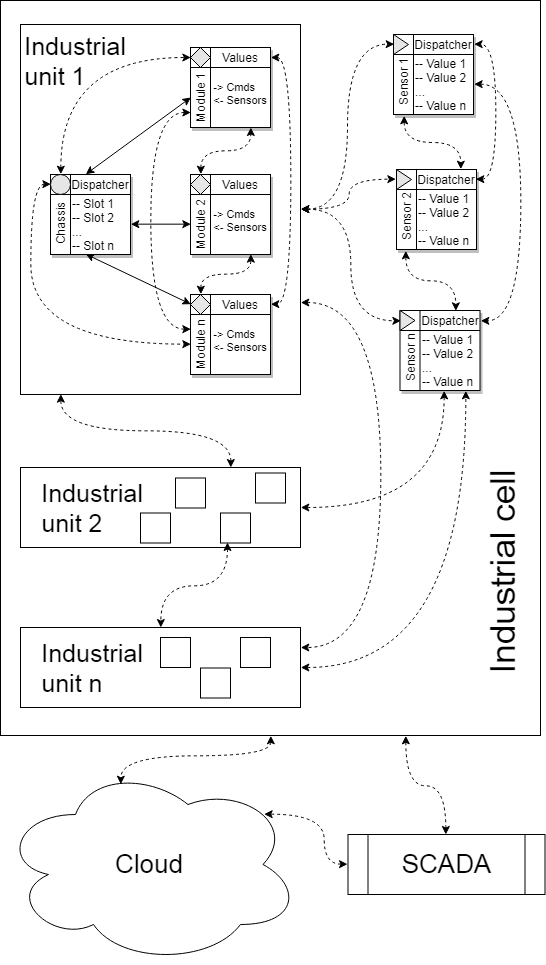
\includegraphics[width=0.5\textwidth]{ch-3/main-arch}
%	}
%	\caption{Слотовая модель модульного оборудования}\label{fig:main-arch}
%\end{figure}

Слот "--- это запись типа <<ключ-значение>>, из которой диспетчер извлекает необходимые данные. Слот включает в себя следующие поля:

\begin{enumerate}
	\item Адрес.
	\item Название модуля/датчика.
	\item Функции.
	\item Возвращаемое значение.
	\item Пределы возвращаемого значения.
\end{enumerate}

В качестве адреса выступают IPv6-адрес и порт, необходимые для взаимодействия с модулем. Название должно быть представлено в строковом виде или числовым идентификатором. Доступные для выполнения функции описываются набором G-кодов и М-функций в соответствии со стандартами ISO 6983-1 и ISO/TR 6983-2.
Например, фрезерный модуль будет представлять возможность работать с командами M3 и M4 (запуск шпинделя по и против часовой стрелки CW/CCW), M5 (останов шпинделя) и S (скорость вращения); для лазерного модуля "--- это будут команды M3 (включить лазер), М5 (выключить) и S (задать мощность в процентах); для магазина инструментов "--- M6 (сменить инструмент) и T (выбрать инструмент из магазина по номеру).  При этом все команды, связанные с перемещением модуля в трёх основных координатах, определяются модулем координатного шасси.

\begin{figure}[ht]
\centerfloat{
	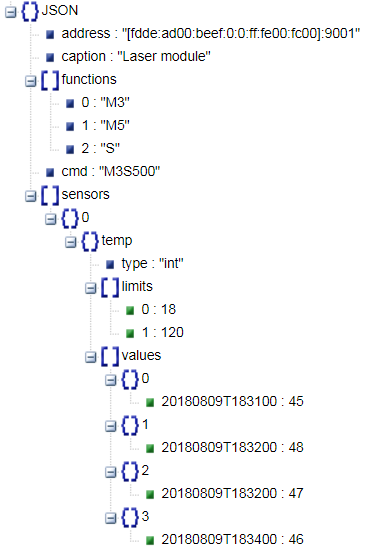
\includegraphics[width=0.5\textwidth]{ch-3/json}
}
\caption{Иерархическая структура единого реестра в формате JSON}\label{fig:json}
\end{figure}

Возвращаемое значение не обязательно должно быть одним. Описание каждого из них включает в себя тип, пределы и массив значений с временными метками. Диспетчер контролирует выход каждого значения за допустимые пределы, и в случае возникновения такой ситуации – осуществляет анализ возникшей ошибки, и принимается решение о возможности или невозможности продолжения работы оборудования.

Рассмотрим теперь процедуру регистрации модуля в реестре диспетчера. С точки зрения протокола "--- здесь нет никаких проблем: сообщения в формате JSON\footnote{В бинарном представлении.} передаются через очередь сообщений с последующей записью в распределенное хранилище. Однако не стоит забывать, что все диспетчеры и все модули находятся в единой самоорганизующейся ячеистой сети. Возникает вопрос "--- как модуль определит к какому конкретно диспетчеру он подключен физически.

Предлагается следующее решение. Физическое подключение каждого модуля реализуется по трехпроводному интерфейсу, где по двум проводникам передается питающее напряжении, а третий используется в качестве линии безопасности. Линия безопасности объединяет все модули одной единицы оборудования по схеме <<монтажное И>>. В данной схеме линия безопасности подтянута резистором к плюсу питания. Так как сопротивление между линией и землей бесконечность, а между питанием и линией равно номиналу резистора, то напряжение на линии равно напряжению питания. То есть высокий уровень или логическая единица. Все модули подключены к линии и могут замыкать её на землю. Соответственно, на линии будет высокий уровень только тогда, когда все модули выставят высокий уровень на своих выходах. Как только любой из модулей соединит линию с землей, на ней установится низкий логический уровень и нb один модуль не сможет на это повлиять.

\begin{figure}[ht]
\centerfloat{
	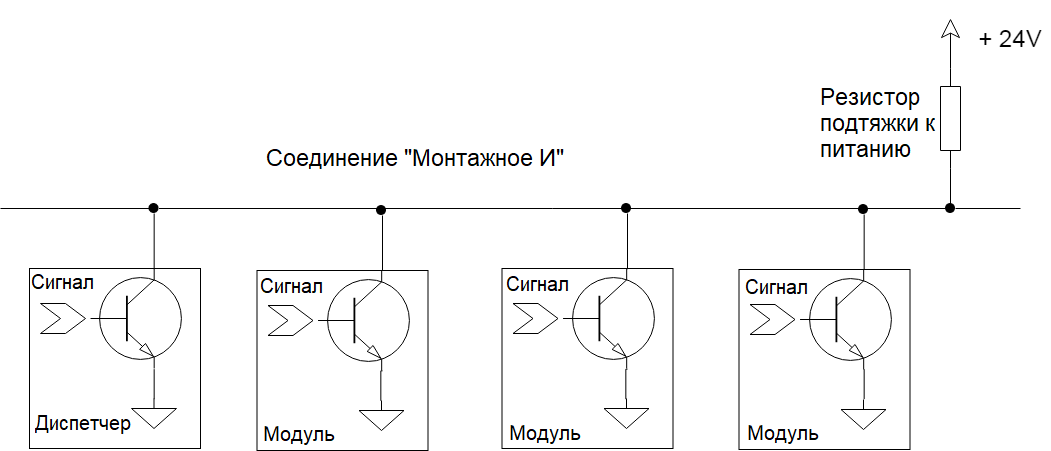
\includegraphics[width=\textwidth]{ch-3/logic-and}
}
\caption{Схема шины безопасности}\label{fig:logic-and}
\end{figure}

Таким образом, основная задача линии безопасности "--- регистрировать аварийные ситуации. В случае возникновения аварии в любом из модулей, он соединяет линию безопасности с землей, что является сигналом для других модулей прекратить работу и перейти в режим восстановления после сбоя. Необходимо отметить, что к этой же линии подключена являющаяся обязательной для любого промышленного оборудования кнопка аварийного останова, а также все концевые выключатели, если они предусмотрены конструкцией.

Кроме всего прочего в процессе инициализации модулей линия безопасности может быть использована для регистрации новых модулей. Вновь подключенный модуль вначале осуществляет подключение к сети OpenThread, затем переводит линию безопасности на низкий логический уровень. Диспетчер детектирует это, после чего получает список всех ближайших к нему узлов (neighbors в терминологии OpenThread), выбирает среди них те, которые имеют статус не подключен, после чего просит первого из них перевести линию обратно на высокий логический уровень. Если уровень изменился, значит диспетчер и модуль подключены к одной линии, следовательно, модуль может быть зарегистрирован в реестре. В противном случае, диспетчер переходит к следующему модулю в списке.

\subsection{Методика определения максимальной пропускной способности канала передачи данных}

Основой предлагаемой сетевой архитектуры является открытый интерфейс, который позволяет аппаратным компонентам оставаться автономными, но в то же время при необходимости обмениваться данными с другими компонентами. Очевидно, что создать такой интерфейс без унификации протокола передачи данных невозможно. Этот протокол должен работать со всеми протоколами и обеспечивать возможность прозрачного обмена информацией между процессами операционной системы, а также между узлами разнородной сети, которые могут действовать как программная служба, работающая под управлением операционной системы и физического контроллера.

Всем этим требованиям удовлетворяют уже упомянутые очереди сообщений. Очередь сообщений "--- это протокол асинхронной связи, поэтому получатель и отправитель не взаимодействуют напрямую, а вместо этого используют очередь сообщений. Очереди сообщений повышают отказоустойчивость системы, поскольку сообщения остаются в очереди и могут обрабатываться даже в случае отказа узла передатчика.

Очереди сообщений гарантируют доставку сообщений, по крайней мере, до тех пор, пока один узел не станет активным и не сможет его обработать, и не нарушают порядок сообщений. Очередь является одновременно и удобным инструментом для реализации сложных асинхронных систем, управляемых сообщениями, и широкой темой в исследованиях в области информатики. Другими словами, очереди рассматриваются с двух сторон.

С одной стороны рассматриваются вопросы оптимизации внутренней организации очереди сообщений. Существует достаточно статей об улучшенных планировщиках очередей, которые были получены модификацией алгоритма очередей~\cite{Valente201416, Rizzo201534}. Например, Кахлон модифицировал алгоритм взвешенной справедливой организации очередей для сети WiMAX, которая содержит как реальный, так и сгенерированный искусственно трафик~\cite{Kahlon2016357}. Кроме того, очереди используются при планировании энергосбережения, поэтому Мэтью Эндрюс и Лиза Чжан предложили адаптивную к скорости версию алгоритма планирования взвешенной справедливой организации очередей и доказали её высокую эффективность~\cite{Andrews2014247}. Чтобы добиться высокой производительности, исследователи начали разработку новых гибридных алгоритмов генетической организации очередей для планирования~\cite{Rashidi2017331, Kahlon2016357}.

С другой "--- решаются некоторые задачи корректного использования очередей сообщений в прикладных приложениях. Например, Дж. Акоста-Кано использует систему очередей сообщений MSMQ и решения, ориентированные на веб-службы, для соединения программного обеспечения цеха с набором производственного оборудования~\cite{AcostaCano2013447}. Для создания корпоративной системы обмена сообщениями Гурсев Сингх Калра использовал ActiveMQ вместе со службой обмена сообщениями Java~\cite{Kalra20147}. Исследователи из Технологического университета Кельце реализовали беспроводную сеть для приложений мобильных роботов с использованием протокола MQTT~\cite{KAZALA2015231}. Кроме того, использование фреймворка ZeroMQ описано в нескольких статьях~\cite{KIRILL2015278, GOERTZEL2014158, ANDREEV201533}. Очереди сообщений стали довольно распространенными и используются во многих сферах, включая производство~\cite{STOCK2014320, MORARIU20121850}.

В данном разделе приводится сравнительный анализ и оценка производительности различных протоколов очереди сообщений для передачи двоичных данных JSON. В настоящее время этот протокол является отраслевым стандартом как для хранения данных, так и для передачи больших данных. Кроме того, он широко используется для создания распределенных сетей Интернета вещей (IoT), а также веб-сервисов. Формат JSON текстовый, что упрощает работу с ним. Существует достаточное количество программных инструментов, позволяющих реализовать двоичную сериализацию JSON, чтобы уменьшить размер сообщения и увеличить очередь сообщений, что увеличивает скорость отклика распределенной системы управления модульным оборудованием.

Очевидно, что распределенная система управления реализуется на базе существующей корпоративной компьютерной сети, состоящей из самых разнообразных компьютеров, программируемых логических контроллеров, контроллеров нижнего уровня, серверов и т.\,д. В качестве среды передачи данных используется скоростное проводное соединение (на основе медных или оптических кабелей) или беспроводное. Это особенно важно на производстве, потому что технологическое оборудование может размещаться в достаточно крупных цехах, где использование только проводной связи экономически нецелесообразно.

Не следует забывать, что корпоративная сеть предприятия может быть территориально распределенной. Сегодня в отрасли все чаще используются облачные технологии для таких задач, как выполнение сложных расчетов, связанных с подготовкой управляющих программ для оборудования с ЧПУ или созданием виртуальных моделей оборудования.

Все это приводит к необходимости экономного использования сетевых ресурсов для достижения максимальной производительности распределенной системы ЧПУ. Цель рассматриваемой методики "--- оценить накладные расходы сети, связанные с упаковкой и распаковкой двоичных данных JSON, а также передать их через очередь сообщений. Будет проведено сравнение пропускной способности очереди сообщений и <<сырых>> TCP-сокетов как для передачи между процессами операционной системы, так и для передачи по различным сетям.

\paragraph{Сетевые сценарии}

Рассмотрены возможные сценарии сетевого взаимодействия компонентов распределенной системы в модульном оборудовании.

\begin{enumerate}
\item\textit{Взаимодействие процессов операционной системы}

Предлагается установка компонентов распределенной системы управления на персональный компьютер (ПК) или универсальный сервер. Были рассмотрены возможности межпроцессного взаимодействия (IPC) для операционных систем, совместимых с POSIX. Этот сценарий является наиболее распространенным при реализации логики высокого уровня. Например, модуль анализа программы управления G-кодом взаимодействует с модулем оптимизацией траектории. Очевидно, что оба этих модуля не решают задачи в реальном времени, и, как правило, их можно установить на обычные ПК.

\item\textit{Взаимодействие аппаратных и программных модулей в неоднородной компьютерной сети}

Это наиболее распространенный сценарий взаимодействия в распределенной сети. Предполагается возможность прозрачной связи между контроллерами нижнего уровня, компьютерами и серверами общего назначения. Каждый из участников этого взаимодействия может выступать как клиент, так и как сервер. Это может быть реализовано как двухточечное или широковещательное соединение. Например, низкоуровневый запрограммированный логический контроллер, который собирает данные с датчиков и передает их в сеть, может выступать в качестве источника данных.

В этом случае все узлы, заинтересованные в получении этих данных, будут действовать как приемники: контроллеры движения, серверы для сбора статистических данных о производственном процессе, интерфейсные модули оператора и т.д. Другой пример "--- видеокамера, транслирующая видеосигнал от область обработки. Этот сигнал может отображаться на физическом мониторе или в виджете пользовательского интерфейса, передаваться в систему машинного зрения для анализа и т.\,д. С другой стороны, специализированные управляющие сигналы передаются непосредственно между двумя заранее определенными узлами.

\item\textit{Взаимодействие с пользователем (оператором)}

Пользовательский интерфейс "--- одна из важнейших частей любой системы управления оборудованием. Использование децентрализованного подхода к проектированию таких систем дает огромные преимущества перед классическими монолитными системами. В классических системах пользовательский интерфейс неотделим от контроллера ЧПУ. В ранних системах ЧПУ взаимодействие с пользователем в основном осуществлялось с помощью физических компонентов управления, таких как кнопки, переключатели, символьные индикаторы и т.\,д. Но в современных системах интерфейс становится виртуальным, то есть отображается на экране системы ЧПУ. Количество физических компонентов управления сокращается, и остаются только компоненты, обеспечивающие безопасность работы (например, кнопка аварийной остановки) или простоту управления (например, джойстик).

Очевидно, что использование виртуального интерфейса, жестко привязанного к контроллеру, неудобно и нецелесообразно. Такие интерфейсы обладают низкой гибкостью, их сложно адаптировать под нужды пользователей, а также практически невозможно организовать удаленное управление. Поэтому для создания интерфейса оператора для распределенной системы управления предполагается использование веб-технологий.

В этом случае основным терминалом управления будет веб-браузер, установленный либо на персональном компьютере, либо на мобильном устройстве. При этом часть вычислительных задач будет передаваться прямо в браузер, для чего требуется возможность получать данные из распределенной сети напрямую через него. Это создает отдельный сетевой сценарий, поскольку клиентские веб-приложения используют собственный стек технологий, которые накладывают определенные ограничения на работу распределенной системы управления модульным оборудованием.

\end{enumerate}

\paragraph{Методика измерения.}
\label{sec:methodology}

Измерения, описанные в этом разделе, осуществлялись путем передачи данных между двумя процессами, подключенными через TCP/IP. Это позволило создать стабильную тестовую среду, позволяющую исключить накладные расходы, связанные с подготовкой данных. Сначала было проведено сравнение способов межпроцессного взаимодействия. Производительность протокола TCP/IP была проанализирована и сравнена с сокетами UNIX и разделяемой памятью. Затем было проведено нагрузочное тестирование каналов для различных сетевых сценариев.

Кроме того, был проведен анализ производительности различных инструментов упаковки/распаковки двоичных данных JSON. После этого был проведен анализ пропускной способности нескольких библиотек очередей сообщений, на основании которого был выбран наиболее производительный вариант. В конце был произведен окончательный расчет максимальной пропускной способности для всех рассматриваемых сетевых сценариев.

\paragraph{Тестовые установки.}

Были использованы четыре тестовых набора, представляющих различные архитектуры и компоненты производительности распределенной системы ЧПУ:

\begin{enumerate}
	\item \textit{Персональный компьютер (сокр. ПК)} "--- это компьютер с низкой производительностью, используемый в распределенной системе ЧПУ для решения широкого круга задач. Технические характеристики: Intel Core i5 CPU M520 @ \SI{2,4}{\giga\hertz}, \SI{4}{\gibi\byte} ОЗУ. Беспроводной сетевой адаптер AR9285 802.11 b/g/n, Yukon Optima 88E8059 Gigabit Ethernet. Операционная система: Ubuntu 16.10, GNU/Linux 4.8.0-41 x86-64.
	
	\item \textit{Портативный персональный компьютер (сокр. ППК)} "---  компьютер, который может использоваться оператором распределенной системы ЧПУ в качестве терминала или для дистанционного управления. Технические характеристики: MacBook Pro, Intel Core i5 CPU @ \SI{2,6}{\giga\hertz}, \SI{8}{\gibi\byte} ОЗУ.
	%, Гигабитная сеть.
	Операционная система: OS X 10.10.5, Darwin 14.5.0.
	\item \textit{Сервер (сокр. СРВ)} "--- это высокопроизводительный компьютер, используемый для наиболее ресурсоемких задач распределенной системы ЧПУ. Технические характеристики: 2 x Intel Xeon E5620 CPU @ \SI{2,4}{\giga\hertz}, \SI{32}{\gibi\byte} ОЗУ.
	%, Гигабитная сеть Intel 82575EB.
	
	\item \textit{Микрокомпьютер (сокр. МПК)} "--- это встроенная система на кристалле, используемая для реализации низкоуровневых алгоритмов в режиме реального времени. Технические характеристики: Amlogic S905 Quad Core Cortex-A53 @ \SI{1,5}{\giga\hertz}, 64-битный процессор ARMv8 ГГц с графическим процессором Mali-450, \SI{2}{\gibi\byte} ОЗУ.
	%, Гигабитная сеть Realtek RTL8211F.
	Операционная система: Ubuntu 16.04 LTS.
	
	\item \textit{Виртуальный сервер (сокр. МСРВ)} "--- это облачная виртуальная машина, используемая для оптимизации вычислительной мощности распределенной системы ЧПУ путем передачи части программных компонентов на выделенные серверы. Технические характеристики: Intel Xeon CPU E5645 @ \SI{2,4}{\giga\hertz}, \SI{512}{\mebi\byte} ОЗУ. Операционная система: Ubuntu Linux 16.04.
\end{enumerate}

\paragraph{Библиотеки и фреймворки.}

Оценка производительности потребовала анализа инструментов разработки (программных библиотек) для упаковки/распаковки двоичных данных JSON и реализации очереди сообщений и выбора из них, наиболее подходящих для решения данной проблемы. Были сформулированы следующие требования к библиотекам и фреймворкам для упаковки/распаковки двоичных данных JSON:

\begin{itemize}
	\item Лицензия с открытым исходным кодом
	\item Поддержка языков программирования C, Python, Go и JavaScript (основных языков программирования, используемых для реализации распределенной системы ЧПУ)
	\item Небольшой объем программной библиотеки
	\item Качественная документация
\end{itemize}


В результате проведенного анализа для тестирования были выбраны следующие библиотеки: MessagePack, BSON, UBJSON, CBOR.

\begin{itemize}
	\item \textit{MessagePack} "--- это формат обмена цифровыми данными, предназначенный для двоичного представления простых структур данных, таких как массивы и ассоциативные массивы.
	\item \textit{BSON} "--- это надмножество JSON, включая дополнительные регулярные выражения, двоичные данные и даты.
	\item \textit{UBJSON} "--- это формат обмена цифровыми данными, имитирующий JSON, который занимает меньше памяти.
	\item \textit{CBOR} "--- это формат обмена цифровыми данными по стандарту ETF RFC 7049.
\end{itemize}


Для тестирования были выбраны следующие библиотеки: ZeroMQ, NanoMsg, RabbitMQ и ActiveMQ. Первые две могут работать без специального брокера сообщений. Для других использование специального брокера сообщений обязательно.

\begin{itemize}
	\item \textit{ZeroMQ} "--- высокопроизводительная асинхронная библиотека сообщений. Она предназначена для использования в распределенных или параллельных приложениях. Она реализует очередь сообщений, но, в отличие от промежуточного программного обеспечения, ориентированного на сообщения, библиотека ZeroMQ может работать без специального брокера сообщений.
	\item \textit{Nanomsg} "--- ответвление ZeroMQ с возможностью подключения пользовательских транспортных протоколов и улучшенной производительностью за счет оптимизации многопоточности.
	\item \textit{RabbitMQ} "--- платформа, которая реализует систему обмена сообщениями между компонентами программного обеспечения на основе стандартного AMQP (Advanced Message Queuing Protocol). Она использует специальный брокер для передачи сообщений.
	Существует реализация клиентов для доступа к RabbitMQ для ряда языков программирования и платформ, широко используемых в веб-разработке.
	\item \textit{ActiveMQ} "--- платформа для обмена сообщениями, которая также использует брокера. Она имеет следующие основные функции: кластеризацию, хранение сообщений, возможность использования различных баз данных, кеширование и ведение журнала.
\end{itemize}

\paragraph{Инструменты.}

Для сравнения пропускной способности в рассматриваемых сетевых сценариях использовались следующие инструменты:

\begin{itemize}
	\item \textit{socat} "--- утилита командной строки, которая создает два двунаправленных байтовых потока и передает данные между ними.
	\item \textit{nc} - это утилита командной строки, которая используется для создания TCP-соединений, отправки UDP-пакетов, прослушивания произвольных TCP- и UDP-портов и сканирования портов.
	\item \textit{iperf} "--- инструмент для измерения пропускной способности сетевых подключений. Он может тестировать пропускную способность TCP или UDP.
	\item \textit{wget} "--- утилита для неинтерактивной загрузки файлов из Интернета, поддерживающая протоколы HTTP, HTTPS и FTP.
	\item \textit{netperf} "--- тест, используемый для измерения различных аспектов производительности сети, особенно при отправке больших объемов данных по TCP или UDP.
	\item \textit{nuttcp} "--- инструмент измерения производительности сети, который позволяет определять пропускную способность данных TCP (или UDP). Отличается возможностью передавать большие объемы данных через буферы в памяти (меньше накладных расходов, более точные измерения).
	\item \textit{nttcp} "--- утилита командной строки, которая позволяет измерять скорость передачи данных в многоадресном соединении (TCP или UDP).
	\item \textit{nload} "--- консольное приложение, которое отслеживает сетевой трафик и использование полосы пропускания в реальном времени. Оно визуализирует входящий и исходящий трафик с помощью графиков и предоставляет дополнительную информацию, такую ​​как общий объем переданных данных и минимальное/максимальное использование сети.
	\item \textit{mpstat} "--- утилита командной строки для сбора статистики об использовании ресурсов центрального процессора.
\end{itemize}

Наборы тестов были разработаны для выполнения автоматических измерений отслеживаемых параметров производительности для трех целевых языков программирования: C, Python и JavaScript. Использовались следующие инструменты разработки:

\begin{itemize}
	\item Интерпретатор Python версии 3.5.2.
	\item Набор инструментов GNU, версия gcc 6.2.0 20161005 (Ubuntu 6.2.0-5ubuntu12).
	\item Веб-браузер Google Chrome, версия 56.0.2924.87 (используется для запуска тестов, написанных на языке программирования JavaScript).
	\item Интегрированная среда разработки JetBrains PyCharm 2016.3 для языка программирования Python (используется для разработки и отладки тестов).
	\item Интегрированная среда разработки JetBrains WebStorm 2016.3 (используется для разработки и отладки тестов, написанных на языке программирования JavaScript).
\end{itemize}

\paragraph{Сравнение пропускной способности сокетов TCP и UNIX.}

Для сравнения пропускной способности сокетов TCP и UNIX использовались следующие способы:

\begin{enumerate}
\setcounter{enumi}{0}
\item Способ 1 (Сп.\,1): утилита \texttt{socat}, перенос из памяти на диск, используется разделяемая память.
\end{enumerate}

\noindent
\begin{lstlisting}
$ sudo dd if=/dev/urandom of=/dev/shm/data.dump bs=1M count=512
$ sudo socat -u -b32768 UNIX-LISTEN:/tmp/unix.sock./data.dump &
$ sudo socat -u -b32768 "SYSTEM: dd if=/dev/shm/data.dump bs=1M count=512" UNIX:/tmp/unix.sock
$ sudo rm -rf/dev/shm/data.dump
\end{lstlisting}

\begin{enumerate}
\setcounter{enumi}{1}
\item Способ 2 (Сп.\,2): утилита \texttt{socat}, перенос из памяти в память, используется общая память.
\end{enumerate}

\noindent
\begin{lstlisting}
$ sudo dd if=/dev/urandom of=/dev/shm/data.dump bs=1M count=512
$ sudo socat -u -b32768 UNIX-LISTEN:/tmp/unix.sock/dev/shm/data.dump.out &
$ sudo socat -u -b32768 "SYSTEM: dd if=/dev/shm/data.dump bs=1M \
count=512" UNIX:/tmp/unix.sock
$ sudo rm -rf/dev/shm/data.dump
$ sudo rm -rf/dev/shm/data.dump.out
\end{lstlisting}

\begin{enumerate}
\setcounter{enumi}{2}
\item  Способ 3 (Сп.\,3): утилита \texttt{socat}, перенос из памяти на нулевое устройство, используется разделяемая память.
\end{enumerate}

\noindent
\begin{lstlisting}
$ sudo dd if=/dev/urandom of=/dev/shm/data.dump bs=1M count=512
$ sudo socat -u -b32768 UNIX-LISTEN:/tmp/unix.sock/dev/null &
$ sudo socat -u -b32768 "SYSTEM: dd if=/dev/shm/data.dump bs=1M \
count=1024" UNIX:/tmp/unix.sock
$ sudo rm -rf/dev/shm/data.dump
\end{lstlisting}

\begin{enumerate}
\setcounter{enumi}{3}
\item  Способ 4 (Сп.\,4): утилита \texttt{socat}, передача из \texttt{/dev/zero} (специальный файл, который предоставляет столько нулевых символов, сколько читается из него) на нулевое устройство.
\end{enumerate}

\noindent
\begin{lstlisting}
$ sudo socat -u -b32768 UNIX-LISTEN:/tmp/unix.sock/dev/null &
$ sudo socat -u -b32768 "SYSTEM: dd if=/dev/zero bs=1M count=512"\
UNIX:/tmp/unix.sock
\end{lstlisting}

\begin{enumerate}
\setcounter{enumi}{4}
\item  Способ 5 (Сп.\,5): утилита \texttt{nc}, передача данных через общий файл.
\end{enumerate}

\noindent
\begin{lstlisting}
(SEND) $ sudo pv /dev/zero | nc -U /tmp/socket
(RECV) $ sudo nc -lU /tmp/socket>/dev/null
\end{lstlisting}

\begin{enumerate}
\setcounter{enumi}{5}
\item  Способ 6 (Сп.\,6): утилита \texttt{iperf}, передача данных через сокет TCP, размер окна TCP \SI{2,5}{\mega\byte}.
\end{enumerate}

\noindent
\begin{lstlisting}
(SEND) $ iperf -s
(RECV) $ iperf -c localhost
\end{lstlisting}

Результаты сравнительного анализа представлены в таблице~\cref{tab:ipc-band}. Можно видеть, что лучший способ межпроцессного взаимодействия в POSIX-совместимых операционных системах "--- использовать сокеты TCP.

\begin{table}[!htb]
\centering
\caption{Сравнение пропускной способности при использовании межпроцессного взаимодействия}
\label{tab:ipc-band}
	\begin{IEEEeqnarraybox} [\IEEEeqnarraystrutmode \IEEEeqnarraystrutsizeadd{2pt}{0pt}]{x/u/Vx/r/v/r/v/r/v/r/v/r/v/r/x}
	\IEEEeqnarraydblrulerowcut \\
	
	&&&& \IEEEeqnarraymulticol{11}{t}{Пропускная способность, Гбит/с} & \\
	
	& \hfill \raisebox{-3pt}[0pt][0pt]{Тестовая установка} \hfill && \IEEEeqnarraymulticol{13}{h}{}%
	\IEEEeqnarraystrutsize{0pt}{0pt} \\
	
	&&&& \hfill \raisebox{-1pt}[0pt][0pt]{Сп.\,1} \hfill &&
	     \hfill \raisebox{-1pt}[0pt][0pt]{Сп.\,2} \hfill &&
	     \hfill \raisebox{-1pt}[0pt][0pt]{Сп.\,3} \hfill &&
	     \hfill \raisebox{-1pt}[0pt][0pt]{Сп.\,4} \hfill &&
	     \hfill \raisebox{-1pt}[0pt][0pt]{Сп.\,5} \hfill &&
	     \hfill \raisebox{-1pt}[0pt][0pt]{Сп.\,6} \hfill &
	\IEEEeqnarraystrutsizeadd{0pt}{2pt} \\
	%
	\IEEEeqnarraydblrulerowcut \\
	
	& ПК  &&& 0,69 && 5,76 && 7,46 && 12,03 && 6,33 && 22,3 & \\
	& ППК &&& 1,79 && 4,47 && 5,98 && 10,18 && 3,65 && 23,2 & \\
	& СРВ &&& 2,41 && 2,76 && 2,75 && 3,23  && 3,13 && 31,6 & \\
	& МПК &&& 1,98 && 1,96 && 2,38 && 2,86  && 2,04 && 4,61 & \\
	%
	\IEEEeqnarraydblrulerowcut \\
	\end{IEEEeqnarraybox}
\end{table}


\paragraph{Определение средней пропускной способности сетевых подключений.}


Для определения средней пропускной способности сетевых подключений использовались следующие способы:

\begin{enumerate}
\setcounter{enumi}{0}
\item Способ 1 (Сп.\,1): HTTP сервер, передано \SI{10}{\giga\byte} данных.
\end{enumerate}

\noindent
\begin{lstlisting}
(SEND) $ dd if=/dev/urandom of="test" bs=1024K count=10000
(SEND) $ sudo python -m SimpleHTTPServer 80
(RECV) $ wget <IP-адрес сервера>/test
\end{lstlisting}

\begin{enumerate}
\setcounter{enumi}{1}
\item  Способ 2 (Сп.\,2): утилита \texttt{iperf}, размер окна TCP \SI{84,3}{\kilo\byte}, \SI{10}{\giga\byte} данных.
\end{enumerate}

\noindent
\begin{lstlisting}
(SEND) $ ipref -s
(RECV) $ ipref -c <send-ip>
\end{lstlisting}

\begin{enumerate}
\setcounter{enumi}{2}
\item Способ 3 (Сп.\,3): утилита \texttt{netperf}, передано \SI{10}{\giga\byte} данных.
\end{enumerate}

\noindent
\begin{lstlisting}
$ netperf -H <любой-IP-адрес в сети> -4 -T TCP_STREAM
\end{lstlisting}

\begin{enumerate}
\setcounter{enumi}{3}
\item Способ 4 (Сп.\,4): утилита \texttt{nuttcp}, передано \SI{10}{\giga\byte} данных.
\end{enumerate}
\noindent
\begin{lstlisting}
(SEND) $ nuttcp -S
(RECV) $ nuttcp -vvv -i1 <send-ip>
\end{lstlisting}

\begin{enumerate}
\setcounter{enumi}{4}
\item Способ 5 (Сп.\,5): утилита \texttt{nttcp}, передано \SI{10}{\giga\byte} данных.
\end{enumerate}

\noindent
\begin{lstlisting}
(SEND) $ nttcp -i
(RECV) $ nttcp -t -T <send-ip>
\end{lstlisting}

Результаты сравнительного анализа представлены в таблице~\cref{tab:network-band}. Очевидно, что использование протокола HTTP приводит к появлению дополнительных накладных расходов, поэтому этот метод исключается из расчета средней пропускной способности.

\begin{table}[!htb]
	\centering
	\caption{Пропускная способность сетевых подключений}
	\label{tab:network-band}
	\begin{IEEEeqnarraybox} [\IEEEeqnarraystrutmode \IEEEeqnarraystrutsizeadd{2pt}{2pt}]{x/u/Vx/r/v/r/v/r/v/r/v/r/v/r/x}
	\IEEEeqnarraydblrulerowcut \\
	
	&&&& \IEEEeqnarraymulticol{11}{t}{Пропускная способность, Мбит/с} & \\
	
	& \hfill \raisebox{-3pt}[0pt][0pt]{Тип соединения} \hfill && \IEEEeqnarraymulticol{13}{h}{}%
	\IEEEeqnarraystrutsize{0pt}{0pt} \\
	
	&&&& \hfill \raisebox{-1pt}[0pt][0pt]{Сп.\,1} \hfill &&
	     \hfill \raisebox{-1pt}[0pt][0pt]{Сп.\,2} \hfill &&
	     \hfill \raisebox{-1pt}[0pt][0pt]{Сп.\,3} \hfill &&
	     \hfill \raisebox{-1pt}[0pt][0pt]{Сп.\,4} \hfill &&
	     \hfill \raisebox{-1pt}[0pt][0pt]{Сп.\,5} \hfill &&
	     \hfill \raisebox{-1pt}[0pt][0pt]{Средн.} \hfill &
	\IEEEeqnarraystrutsizeadd{0pt}{2pt} \\
	%
	\IEEEeqnarraydblrulerowcut \\
	
	& Беспроводное соединение \rlap{\textsuperscript{1}} &&& 5.25 && 5.95 && 8.00 && 6.86 && 5.47 && 6.57 & \\
	
	& Кабельное соединение \rlap{\textsuperscript{1}} &&& 559.00 && 941.00 && 907.77 && 941.27 && 940.72 && 932.69 & \\
	
	& Облачное соединение \rlap{\textsuperscript{2}} &&& 12.44 && 13.70 && 13.67 && 13.60 && 14.42 && 13.85 & \\
	%
	\IEEEeqnarraydblrulerowcut \\& \IEEEeqnarraymulticol{13}{s}{\scriptsize \textsuperscript{1} Cоединение между \textit{ПК} и \textit{СРВ} в локальной сети.} \\
    & \IEEEeqnarraymulticol{13}{s}{\scriptsize \textsuperscript{2} Cоединение между \textit{СРВ} и \textit{ВСРВ} через Интернет.}%
	\end{IEEEeqnarraybox}
\end{table}


\paragraph{Оценка производительности упаковщиков JSON.}


На рисунке~\cref{fig:json-compress} показана зависимость степени сжатия от размера файла JSON. Файлы JSON состоят из упорядоченного списка элементов. Каждый элемент состоит из имени поля и значения. Имена полей представляют собой строки. Значения включают числа, строки, логические значения или пустые объекты. Все тесты написаны на Python. Из рисунка видно, что для всех библиотек практически не наблюдается зависимости степени сжатия от размера файла JSON.

\begin{figure}[!htb]
	\centering
	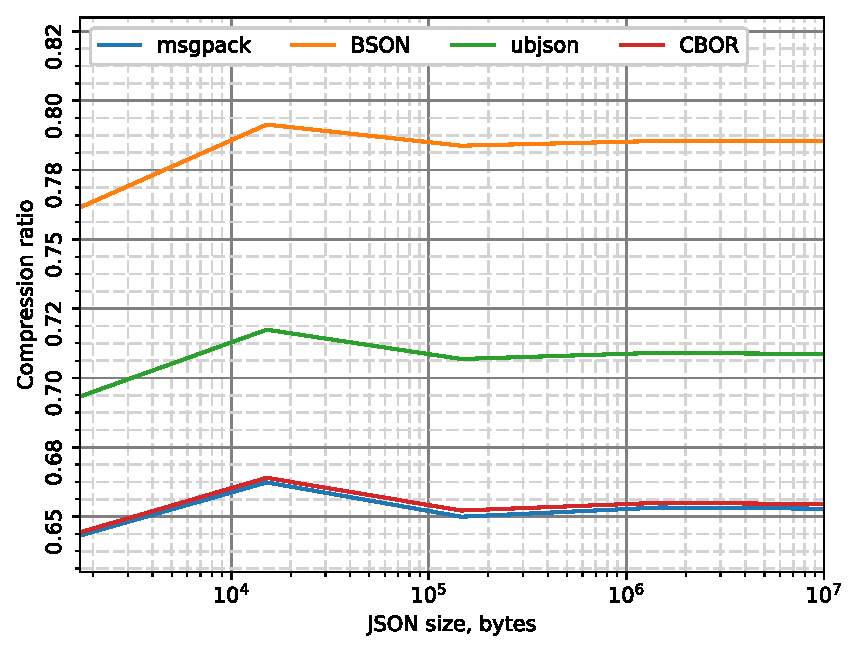
\includegraphics[width=0.7\textwidth]{ch-3/json-compession}
	\caption{Степень сжатия как функция размера файла JSON}
	\label{fig:json-compress}
\end{figure}


Затем была получена зависимость скорости упаковки/распаковки от размера файла JSON. Результаты показаны на рисунках~\cref{fig:json-pack} и \cref{fig:json-unpack}. Как видно, для всех рассмотренных библиотек эта зависимость линейная. Библиотека CBOR показала лучшее время как для упаковки, так и для распаковки.
Следующим шагом было тестирование производительности библиотек CBOR, написанных на разных языках программирования. Произошло 1000 циклов упаковки/распаковки; размер исходного файла JSON был 15\:МБ. Результаты тестирования представлены в таблице~\cref{tab:cbor}.

\begin{figure}[!ht]
	\centering
	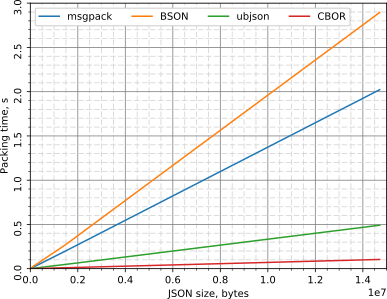
\includegraphics[width=0.7\textwidth]{ch-3/json-pack}
	\caption{Время упаковки в зависимости от размера файла JSON}
	\label{fig:json-pack}
\end{figure}

\begin{figure}[!ht]
	\centering
	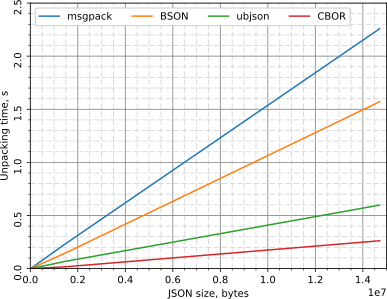
\includegraphics[width=0.7\textwidth]{ch-3/json-unpack}
	\caption{Время распаковки как функция размера файла JSON}
	\label{fig:json-unpack}
\end{figure}

\begin{table}[!htb]
\centering
\caption{Пропускная способность при использовании библиотек CBOR}
\label{tab:cbor}
	\begin{IEEEeqnarraybox} [\IEEEeqnarraystrutmode \IEEEeqnarraystrutsizeadd{2pt}{0pt}]{x/s/Vx/r/v/r/x}
	\IEEEeqnarraydblrulerowcut \\%
	%
	&&&& \IEEEeqnarraymulticol{3}{t}{Пропускная способность, Мбит/с} & \\
	%
	& \hfill \raisebox{-3pt} [0pt] [0pt]{Библиотека} \hfill && \IEEEeqnarraymulticol{5}{h}{}%
	
	\IEEEeqnarraystrutsize{0pt}{0pt} \\
	
	&&&& \hfill \raisebox{-1pt}[0pt][0pt]{Упаковка} \hfill &&
	\hfill \raisebox{-1pt}[0pt][0pt]{Распаковка} \hfill &
	\IEEEeqnarraystrutsizeadd{0pt}{2pt} \\
	%
	\IEEEeqnarraydblrulerowcut \\
	& Python 3.5.2 CBOR &&& 112.73 && 19.13 & \\
	& Python 3.5.2 CBOR2 &&& 7.59 && 4.30 & \\
	& C libcbor (GCC 6.2.0 20161005) &&& 244.13 && 273.07 & \\
	& JavaScript cbor (Chrome 56.0.2924.87) &&& 76.19 && 100.21 & \\
	\IEEEeqnarraydblrulerowcut \\
	\end{IEEEeqnarraybox}
\end{table}
%
\paragraph{Оценка производительности протоколов очереди сообщений.}

Рисунок~\cref{fig:qm-bandwidth} показывает зависимость пропускной способности от размера сообщения. Для каждого метода было передано один миллион сообщений, и используется межпроцессное взаимодействие. По результатам анализа можно сделать вывод, что наиболее рациональный размер сообщения составляет от \SI{1}{\kilo\byte} до \SI{100}{\kilo\byte}.
Библиотеки~NanoMsg и ZeroMQ показали лучшую производительность. NanoMsg был выбран в качестве основного протокола передачи сообщений в рассматриваемой распределенной системе ЧПУ. Основные причины этого решения - лучшая совместимость с POSIX и более гибкий API.

В таблице~\cref{tab: nanomsg} показаны результаты измерения пропускной способности протокола NanoMsg для различных сетевых подключений. Все тесты были написаны на Python, где размер сообщения \SI{1}{\kilo\byte}, и в каждом тесте было отправлено один миллион сообщений.

\begin{table}[!htb]
\centering
\caption{Пропускная способность при использовании протокола NanoMsg}
\label{tab:nanomsg}
	\begin{IEEEeqnarraybox} [\IEEEeqnarraystrutmode \IEEEeqnarraystrutsizeadd{2pt}{0pt}]{x/u/Vx/r/v/r/x}
	\IEEEeqnarraydblrulerowcut \\%
	%
	&&&& \IEEEeqnarraymulticol{3}{t}{Пропускная способность, Мбит/с} & \\
	%
	& \hfill \raisebox{-3pt}[0pt][0pt]{Библиотека} \hfill && \IEEEeqnarraymulticol{5}{h}{}%
	
	\IEEEeqnarraystrutsize{0pt}{0pt} \\
	
	&&&& \hfill \raisebox{-1pt}[0pt][0pt]{Nanomsg PUBSUB} \hfill &&
	\hfill \raisebox{-1pt}[0pt][0pt]{Nanomsg BUS} \hfill &
	\IEEEeqnarraystrutsizeadd{0pt}{2pt} \\
	%
	\IEEEeqnarraydblrulerowcut \\
	& Беспроводное соединение &&& 5.93 && 7.34 & \\
	& Кабельное соединение &&& 880.74 && 880.38 & \\
	& Облачное соединение &&& 15.18 && 14.98 & \\
	\IEEEeqnarraydblrulerowcut \\
	\end{IEEEeqnarraybox}
\end{table}


\begin{figure}[!htb]
	\centering
	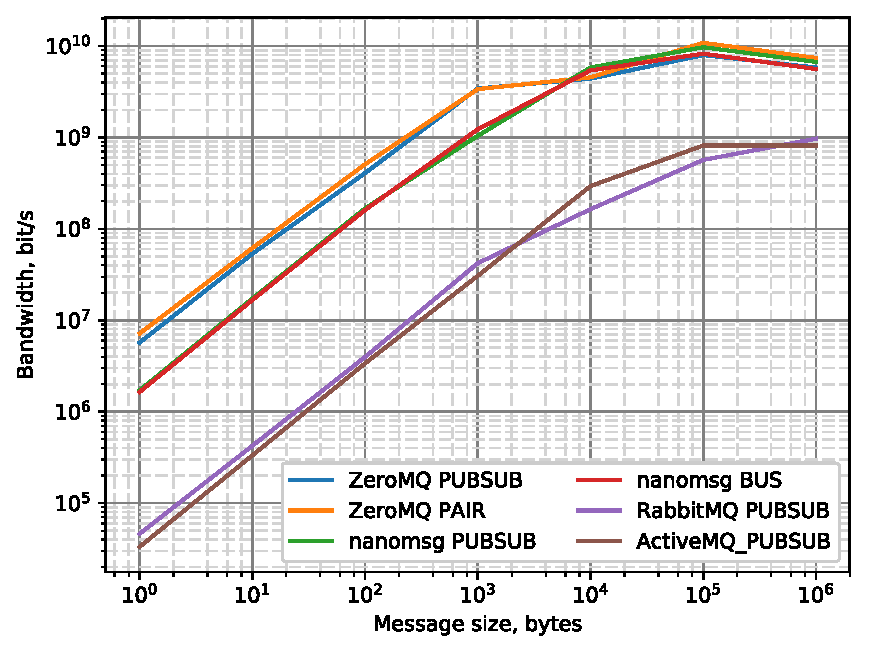
\includegraphics[width=0.9\textwidth]{ch-3/qm-bandwidth}
	\caption{Пропускная способность протоколов очереди сообщений в зависимости от размера сообщения}
	\label{fig:qm-bandwidth}
\end{figure}

\paragraph{Общая оценка производительности.}

Чтобы дать общую оценку производительности протокола очереди сообщений, предлагается использовать формулу для средней полосы пропускания~\cref{eq:example}.

\begin{equation}
\begin{split}
	\label{eq:example}
	\mathcal{B}_a = \frac{\mathcal{M}}{t}
	= \frac{\mathcal{M}}{t_p + t_t + t_u}
	= \frac{\mathcal{M}}
	{\mathcal{M} / \mathcal{S}_p + 
		\gamma\mathcal{M} / \mathcal{B}_t + 
		\mathcal{M} / \mathcal{S}_u} = \\
	= \frac{\mathcal{M}}
	{\frac{\mathcal{M}_(\mathcal{B}_t\mathcal{S}_u) +
			\gamma
			\mathcal{M}(\mathcal{S}_p\mathcal{S}_u) +
			\mathcal{M}(\mathcal{S}_p\mathcal{B}_t)} 
		{\mathcal{S}_p\mathcal{B}_t\mathcal{S}_u}
	}
	=\frac{\mathcal{S}_p\mathcal{B}_t\mathcal{S}_u}
	{\mathcal{B}_t\mathcal{S}_u + \gamma\mathcal{S}_p\mathcal{S}_u + \mathcal{S}_p\mathcal{B}_t}\,,
\end{split}
\end{equation}

\noindent где ${\mathcal{M}}$ "--- размер сообщения, $t$ "--- общее время между двумя точками, $t_p$ "--- время упаковки, $t_t$ "--- время передачи, $t_u$ "--- время распаковки, $\mathcal{S}_p$ "--- скорость упаковки данных JSON, $\mathcal{S}_u$ "--- скорость распаковки данных JSON, $\mathcal{B}_t$ "--- пропускная способность очереди сообщений, $\gamma$ "--- степень сжатия JSON.

Часто библиотеки Python демонстрируют производительность, примерно равную производительности библиотек C. Это связано с тем, что эти библиотеки являются оболочками библиотек C. В этом случае использование библиотек Python предпочтительнее из-за более простого синтаксиса языка программирования Python. Однако рассматриваемые библиотеки Python не показали достаточной производительности, поэтому очевидно, что для реализации серверной части была выбрана библиотека C. При реализации клиентской части использовалась библиотека JS, так как это единственный вариант реализации программ в браузере.

В таблице~\cref{tab:res} показаны результаты расчетов. Расчеты показывают, что средняя полоса пропускания описанного канала связи находится в диапазоне от \SI{6}{\percent} (наихудший случай, упаковка/распаковка требуется на обеих конечных точках) до \SI{95}{\percent} (лучший случай, упаковка/распаковка вообще не требуется, обе конечные точки используют двоичные данные JSON, что подразумевает возможность сжатия сообщений из-за того, что двоичный формат JSON занимает меньше места по сравнению с текстовым JSON).

\begin{table}[!htb]
\centering
\caption{Пропускная способность, кабельное соединение, $\gamma=0,65$}
\label{tab:res}
	\begin{IEEEeqnarraybox} [\IEEEeqnarraystrutmode \IEEEeqnarraystrutsizeadd{2pt}{0pt}]{x/u/Vx/r/v/r/v/r/x/}
	\IEEEeqnarraydblrulerowcut \\
	
	& \hfill %\raisebox{0pt}[0pt][0pt]{Отношение $\mathcal{S}_u / \mathcal{S}$}
	\hfill && \IEEEeqnarraymulticol{0}{h}{}%
	\IEEEeqnarraystrutsize{0pt}{0pt} \\
	
	&&&& \hfill \raisebox{0pt}[0pt][0pt]{Библиотека JS} \hfill &&
	     \hfill \raisebox{0pt}[0pt][0pt]{Библиотека C} \hfill &&
	     \hfill \raisebox{0pt}[0pt][0pt]{Без распаковки} \hfill &
	\IEEEeqnarraystrutsizeadd{0pt}{2pt} \\
	%
	\IEEEeqnarraydblrulerowcut \\
	
	& Библиотека JS &&& n/a \rlap{\textsuperscript{1}} && {57.06} && 70.94 & \\
	& &&& &&{(6.22\,\%)} && (7.60\,\%) & \\
	
	& Библиотека  C &&& 67.50 && 117.70 && 203.18 & \\
	& &&& (7.24\,\%) && (12.62 \,\%) && (21.78 \, \%) & \\
	
	& Без упаковки &&& 93.31 && 227.27 && {954,98} & \\
	& &&& (10.00\,\%) && (24.37\,\%) && {(95,28\,\%)} & \\
	%
	\IEEEeqnarraydblrulerowcut \\
	& \IEEEeqnarraymulticol{9}{s}{\scriptsize\textsuperscript{1} Cвязь между клиентами не реализована в рассматриваемом сценарии.}%
	\end{IEEEeqnarraybox}
\end{table}

\subsection{Методика оценки качества сигнала при беспроводном соединении модулей}

Наиболее узким местом в рассматриваемой информационной модели является передача данных по беспроводному каналу в условиях промышленного производства. Поэтому в данном разделе будет рассмотрена методика оценки качества соединения при использовании модулей беспроводной связи, в частности оценено влияние факторов производственной среды, которые могут привести к ухудшению связи и способов их устранения. В производстве присутствуют факторы, способные повлиять на помехозащищенность беспроводного сигнала. Поэтому проводятся различные исследования влияния производственной среды на беспроводной сигнал и определяются критерии его оценки. Например, шведские исследователи оценили влияние электромагнитного шума в цехах для различных диапазонов частот беспроводного сигнала~\cite{6525614, 5475862}. В ходе исследования они определили профиль снижения мощности в различных производственных помещениях с разными уровнями отражения и поглощения сигнала. Аналогичные исследования проводились также в Пекинском университете Цзяотун~\cite{Li2019}, где анализировались амплитудно-временные характеристики электромагнитных шумов на частотах 315, 433 и \SI{916}{\mega\hertz}, возникающих во время сварочных работ.
	
Также в работе~\cite{Girs2013DesignOC} описывается установка для измерения параметров беспроводного сигнала в диапазоне~\SI{2,4}{\giga\hertz}, а также методика измерения. Используя эту установку, учёные получили зависимость между стабильностью беспроводного сигнала и временем, необходимым для передачи стандартного пакета IEEE 802.15.4. В статье~\cite{8308609} рассматривается проблема шумового загрязнения в диапазоне~\SI{2,4}{\giga\hertz} другими сетями и источниками помех. Предложена математическая модель электромагнитного шума в этом диапазоне, которую можно использовать для предварительной оценки помехозащищенности производственных помещений.

Производство обычно рассматривается как иерархическая система, состоящая из уровней, как показано на~\cref{ch-3/fig-1}. На каждом уровне есть элементы сетевой инфраструктуры, обеспечивающие как горизонтальную, так и вертикальную передачу данных.
При этом типы используемых компьютерных сетей различаются на разных уровнях. Это происходит из-за того, что в зависимости от положения в иерархической системе выдвигаются различные требования к скорости передачи данных, безопасности, ширине канала, топологии, надежности и энергоэффективности. Более того, различные компьютерные сети могут сосуществовать на одном уровне в зависимости от выполняемых задач. Поэтому сетевая инфраструктура предприятия является гибридной.

\begin{figure*} [tb]
	\centering
	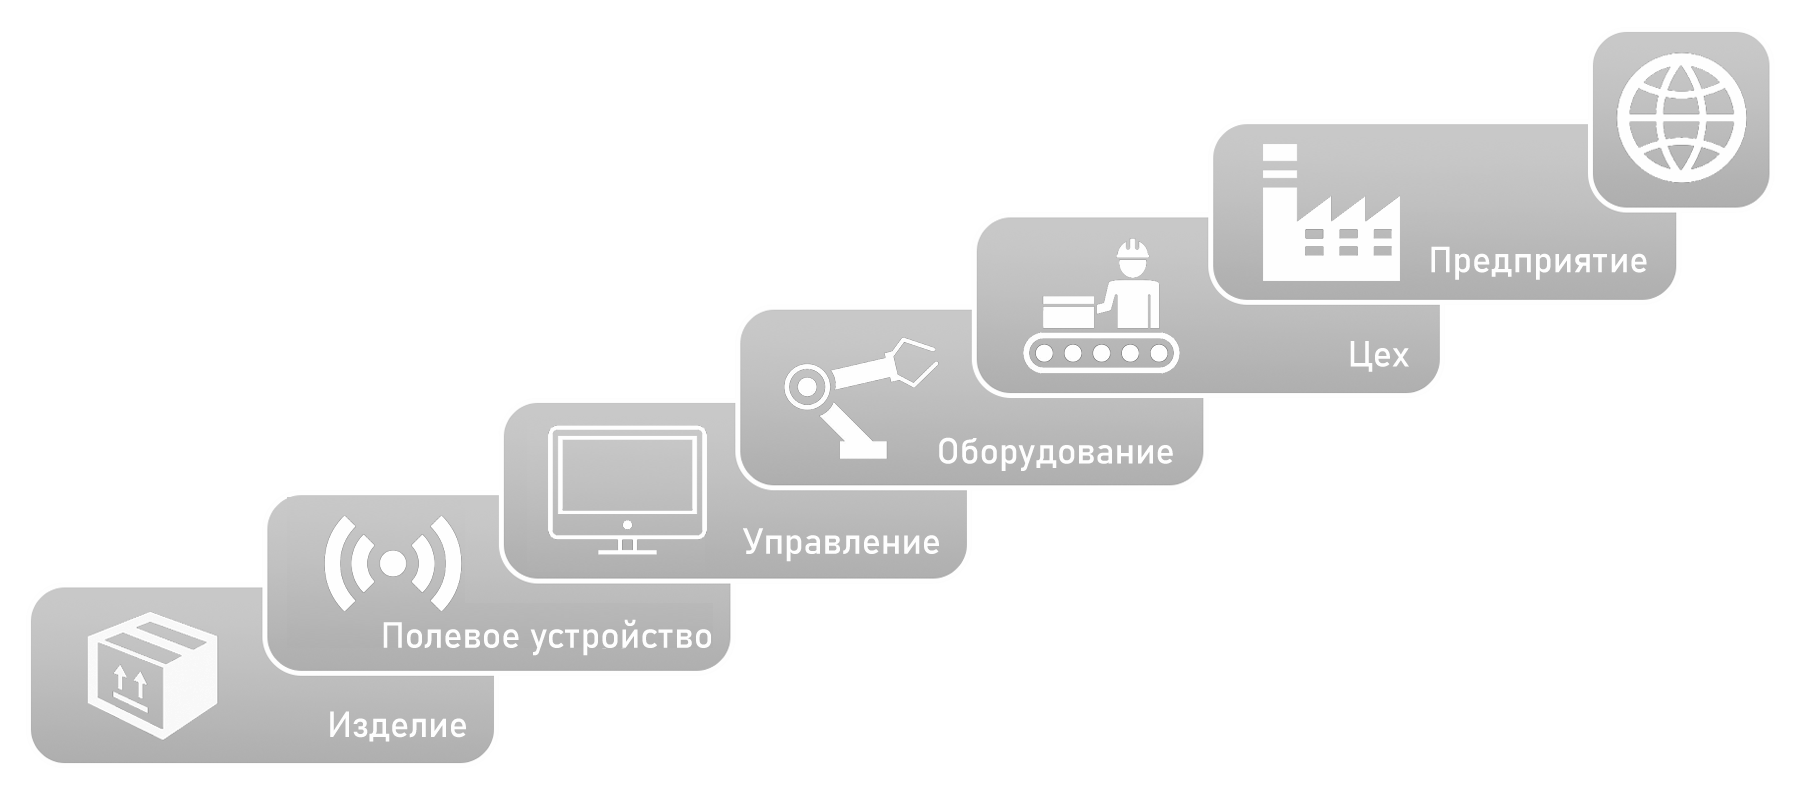
\includegraphics[width=0.9\linewidth]{ch-3/fig-1-ru}
	\caption{Уровни производственной системы}
	\label{ch-3/fig-1}
\end{figure*}

Беспроводные персональные вычислительные сети используются на уровнях системы управления оборудования, производственной ячейки, цеха и, реже, в случае малых предприятий, на уровне всего предприятия. WPAN имеют широкое покрытие и применимы в производственной среде благодаря активной поддержке комитета IEEE (Институт инженеров по электротехнике и электронике). Это привело к появлению ряда технологий, охватываемых набором стандартов IEEE 802.15.4, включая хорошо известные технологии, такие как Bluetooth, ZigBee и Thread.

Одновременно стремительно растет аппаратная база. В настоящее время на рынке представлен большой выбор микросхем и готовых плат, поддерживающих сразу несколько технологий WPAN. Несмотря на изначально небольшую дальность передачи сигнала, использование ячеистой топологии позволяет достичь практически неограниченного диапазона. Также стоит отметить возможность построения WPAN на основе стека TCP/IP, что удобно при работе с другими сетями.

К недостаткам WPAN можно отнести частотные диапазоны, в которых работают эти сети: \SI{868}{\mega\hertz}, \SI{915}{\mega\hertz} и \SI{2,4}{\giga\hertz}. В России они не лицензированы, но имеют ограничения по мощности передатчика~\cite{freq}. Эти диапазоны называются <<частотами ISM>>.\footnote{Сокр. от англ. \textit{Industrial, Scientific, Medical}.} Как следует из названия, большое количество оборудования работает в диапазонах, которые могут создавать помехи сети~\cite{750064, 6209430}.

На производственной площадке существует множество факторов, которые могут ослабить и исказить беспроводной сигнал. Их выявление перед развертыванием беспроводной сети является обязательной процедурой. Рисунок~\cref{ch-3/fig-2} представляет классификацию негативных факторов. Некоторые из этих факторов можно определить заранее уже на этапе разработки компоновки оборудования и агрегатов. Например, тип среды может определяться функциональным назначением производственного помещения. Зная окончательную компоновку блоков, можно определить, где офисные сети Wi-Fi~2,4\,ГГц будут пересекаться с промышленной беспроводной сетью. Учитывая это, можно вносить коррективы, чтобы повысить помехозащищенность сети.

\begin{figure*}[ht]
	\centering
	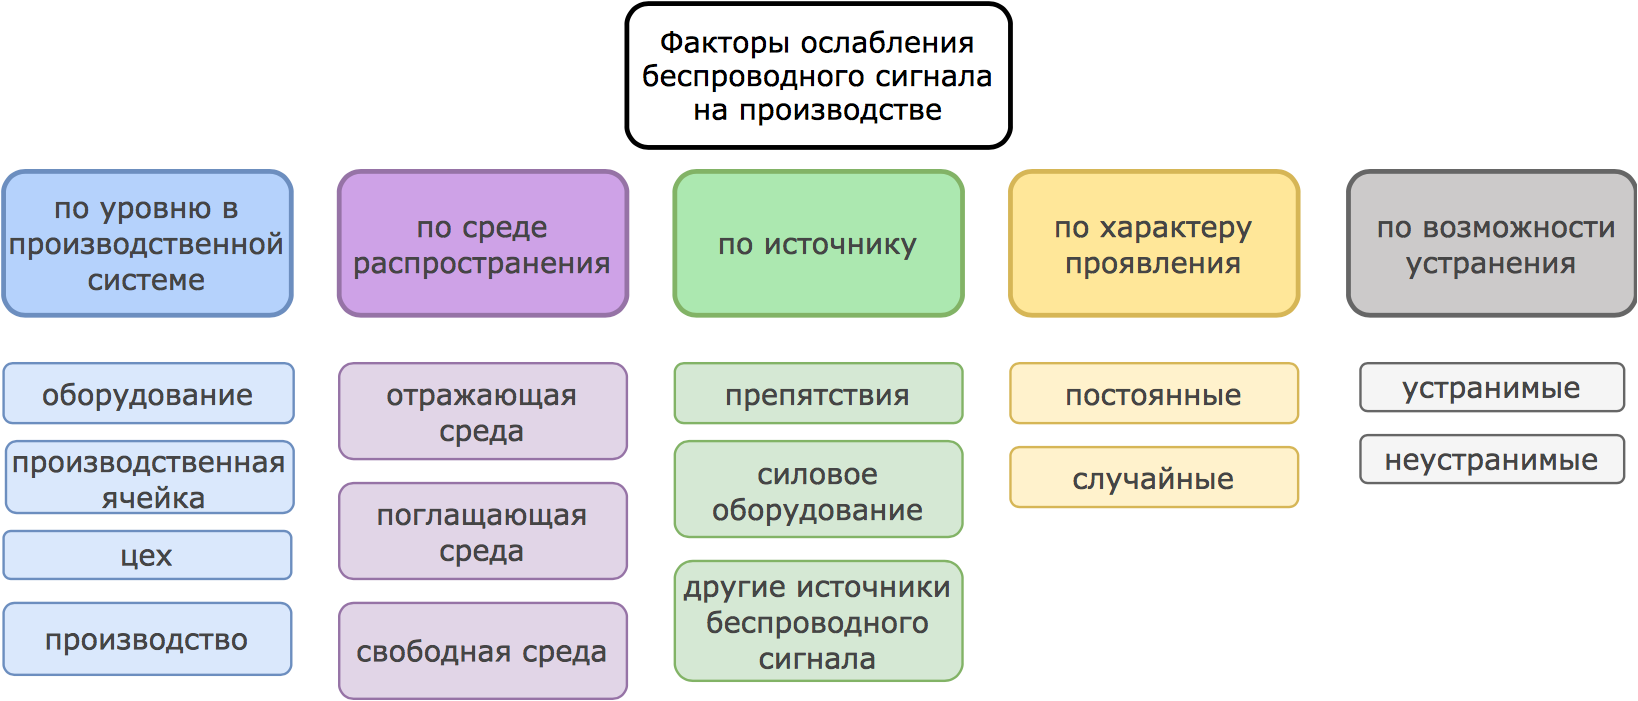
\includegraphics[width=\linewidth]{ch-3/fig-2-ru}
	\caption{Классификация производственных факторов, влияющих на прохождение радиосигнала}
	\label{ch-3/fig-2}
\end{figure*}

Однако развертывание новой беспроводной сети на уже существующей производственной площадке в настоящее время является более актуальной задачей. Кроме того, для получения достаточно точной картины измерения следует проводить непосредственно на предприятии. Для определения качества сигнала используются различные характеристики. Они включают профиль ослабления мощности, амплитудные и временные характеристики, отношение сигнал/шум~\cite{6133782} и т.\,д. К~сожалению, измерение этих параметров требует использования дорогостоящих инструментов "--- анализатора спектра, вектора анализатор цепей и специальные антенны. А квалификационные требования к человеку, производящему измерения, очень высоки.

В предлагаемой методике используется индикатор уровня принимаемого сигнала (RSSI). Его главное преимущество "--- встроенная поддержка практически на любом сетевом оборудовании, включая аппаратную платформу, используемую в эксперименте. Это означает, что можно получить значение RSSI от приемника без использования дополнительного измерительного оборудования. Однако RSSI нельзя использовать напрямую для измерения качества беспроводного сигнала, поскольку этот параметр может содержать значительный компонент помех. Таким образом, сильные помехи могут привести к потере пакетов при увеличении значения RSSI~\cite{8211460}.

Одновременно рассчитывается параметр $RSSI_T$, основанный на характеристиках антенн приемника и передатчика, а также с учётом частоты беспроводного сигнала и опорного параметра затухания~\cref{eq-1, eq-2, eq-3}:

\begin{equation}
	RSSI_T = A-10 \mu\log (d),
	\label{eq-1}
\end{equation}

\noindent где $d$ "--- расстояние от источника, м; $\mu$ "--- показатель ослабления, $\mu = 2$;

\begin{equation}
	A = P_{out} + G_{tx} + G_{rx} -FSPL,
	\label{eq-2}
\end{equation}

\noindent где $P_{out}$ "--- выходная мощность передатчика, дБм; $G_{tx}$ "--- усиление исходной антенны, дБи; $G_{rx}$ "--- усиление антенны приемника, дБи; $FSPL$ "--- потери на трассе в свободном пространстве, дБ;

\begin{equation}
	FSPL = 10 \log (d) +20 \log (f) +20 \log (4 \pi/c),
	\label{eq-3}
\end{equation}

\noindent где $f$ "--- частота, Гц; $c = 299792458$ м/с.

Поэтому в предлагаемом методе используется отклонение $\Delta RSSI$, полученное как разница между измеренным значением $RSSI_P$ и теоретическим значением $RSSI_T$~ \cref{eq-4}.

\begin{equation}
	\Delta RSSI = RSSI_T-RSSI_P
	\label{eq-4}
\end{equation}

Тем не менее, при проектировании сети, особенно в случае применения ячеистой топологии, сначала определяется расположение узлов в помещении. Следовательно, можно перейти от отклонения $\Delta RSSI$ к максимальному расстоянию между узлами~$D_{max}$~\cref{eq-5}, более удобному параметру для рассматриваемой задачи. Сигнал со значением RSSI менее~-80\,дБм считается слабым~\cite{mob_sig}. На основе этого утверждения и~\cref{eq-4} можно рассчитать $RSSI_T$~\cref{eq-6} на определенном расстоянии от передатчика с учетом среднего отклонения $\Delta RSSI$, на который влияют факторы конкретной производственной среды~\cref{eq-7}.

\begin{equation}
	D_{max} = 10^\frac{A-RSSI_T}{10 \mu}
	\label{eq-5}
\end{equation}

\begin{equation}
	RSSI_T = -80-\overline{{\mathit \Delta} RSSI}
	\label{eq-6}
\end{equation}

\begin{equation}
	\overline{{\mathit \Delta} RSSI} = \frac1n \sum_{\substack{0 < i < n}}{\mathit\Delta} RSSI_i,
	\label{eq-7}
\end{equation}

\noindent где $n$ "--- количество измерений. В этом случае $n = 25$.

\paragraph{План эксперимента.}

Эксперимент проводился для определения существенных факторов, ослабляющих беспроводной сигнал в производственной среде. Для этого необходимо было собрать набор экспериментальных данных и оценить помехозащищенность WPAN под влиянием заданных факторов в соответствии с разработанной методикой.
Измерения были получены с использованием экспериментальной установки, показанной на~\cref{ch-3/fig-3}.

\begin{figure} [ht]
	\centering
	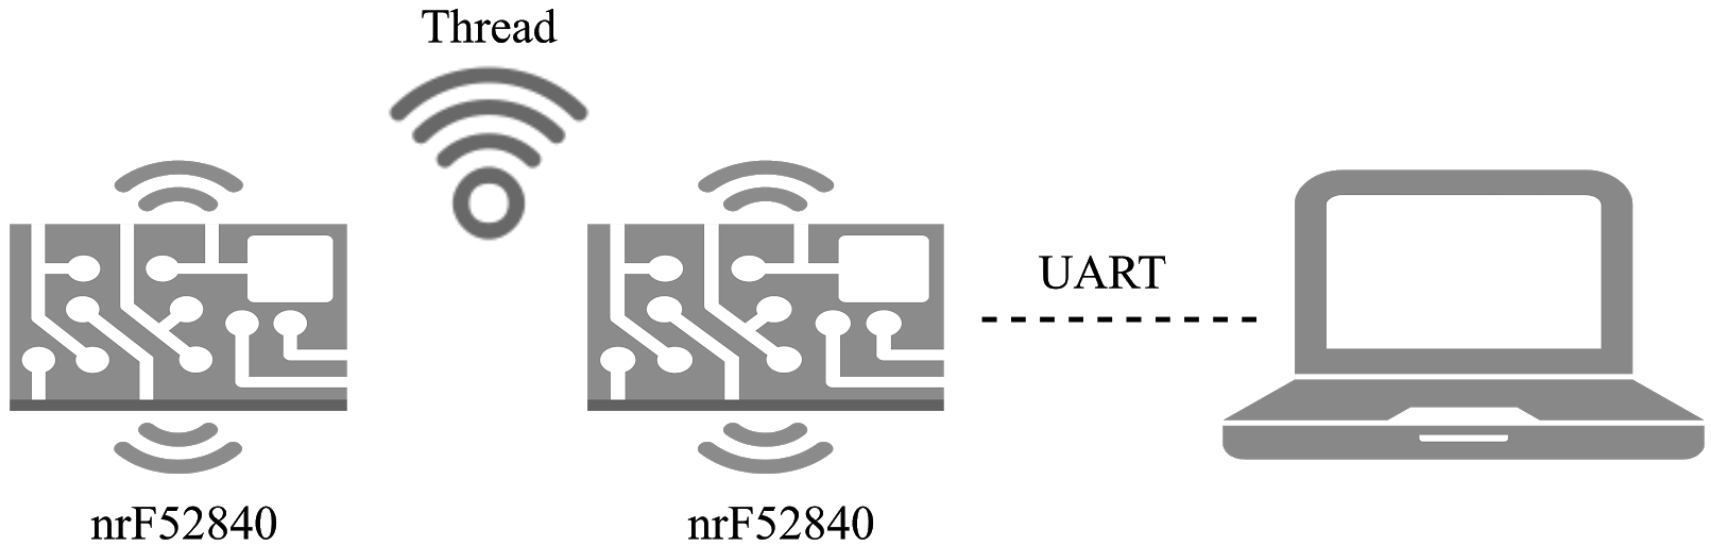
\includegraphics[width=\linewidth]{ch-3/fig-3}
	\caption{Экспериментальная установка}
	\label{ch-3/fig-3}
\end{figure}

Установка состоит из двух плат на базе микросхемы nRF52840\footnote{Электронный ресурс: {\url{https://wiki.makerdiary.com/nrf52840-mdk-usb-dongle/}} (дата обращения: 16.07.2020).}, которые действуют как приемник и передатчик. На плате установлена чип-антенна ACA-2012-A1-CC-S.\footnote{Электронный ресурс: \url{https://www.endrich.com/fm/2/ACA-2012-A1-CC-S.pdf} (дата обращения 23.02.2020).}
%параметры которой указаны в таблице~\cref{tab-1}.
Кроме того, для регистрации данных используется персональный компьютер. Персональный компьютер подключен к приемнику через интерфейс универсального асинхронного приемника-передатчика (UART) для получения измеренных значений RSSI. Внутри WPAN сообщение передается по протоколу Thread.\footnote{Электронный ресурс: {\url{https://openthread.io}} (дата обращения: 20.05.2020).}

Эксперимент проводился на производственных площадях компании <<Лар Технологии>>, специализирующейся на разработке технологического оборудования. Влияние каждого из следующих факторов, выбранных в соответствии с классификацией в~\cref{ch-3/fig-2}, изучалось отдельно.

\begin{itemize}
\item склад металлопроката;\footnote{Как фактор отражающей среды.}
\item силовое оборудование:
	\begin{itemize}
		\item асинхронный двигатель;
		\item шаговый двигатель;
		\item сварочный аппарат;
	\end{itemize}
\item толстостенная стальная труба (толщина стенки~\SI{20}{\milli\meter}) как фактор препятствия;
\item сети (Wi-Fi и ZigBee).
\end{itemize}

Значения RSSI под воздействием сетей~\SI{2,4}{\giga\hertz} были зафиксированы в офисном помещении, так как их не было в производственных помещениях. Также были получены измерения на открытом воздухе без влияния перечисленных факторов. Эксперимент проводился в диапазоне от 0,5 до \SI{24,5}{\meter} с шагом \SI{1}{\meter}. На каждом шаге выполнялась серия измерений в течение одной минуты с периодом~\SI{1}{\second}.

\paragraph{Результаты экспериментов.}

%\begin{table}[!h]
%	\centering
%	\caption{Спецификация чип-антенны ACA-2012-A1-CC-S} \vspace{4pt}
%	\label{tab-1}
%	\begin{tabularx}{\linewidth}{XX}
%		\toprule
%		\textbf{Параметр} & \textbf{Значение} \\
%		\midrule
%		Диапазон частот (МГц) & 2400--2483 \\
%		Коэффициент стоячей волны &$<$3,0\\
%		Поляризация & линейная \\
%		Входное сопротивление (Ом) & 50 \\
%		Коэффициент усиления (дБи) & 1,72 \\
%		Размеры (мм) & 2,0 $\times$ 1,2 $\times$ 0,55\\
%		\bottomrule
%	\end{tabularx}
%\end{table}

По мере увеличения расстояния между приемником и передатчиком значение RSSI уменьшается, что можно объяснить явлением потерь на пути распространения. В этом случае значение RSSI уменьшается логарифмически в зависимости от расстояния~\cref{eq-1}. Это происходит в соответствии с законом сохранения энергии. Поскольку волна передает энергию и распространяется сферически, энергия с увеличением расстояния распределяется по увеличивающейся площади поверхности сферы.~\footnote{Электронный ресурс: {\tiny\url{http://asupro.com/gps-gsm/means-identification/automatic/linear-circular-polarization-rfid-system.html}} (дата обращения: 09.05.2020).} Рисунок~\cref{ch-3/fig-4a} показывает график, отражающий теоретическую кривую значений RSSI, полученных в соответствии с~\cref{eq-1}, и зависимость между RSSI и расстоянием при измерениях на открытом воздухе. Можно отметить, что кривые оказались похожими по форме. Однако есть небольшие отклонения RSSI, значения которых показаны в~\cref{ch-3/fig-4b}.

\begin{figure}[!htb]
	\centering
	\subfloat []{%
		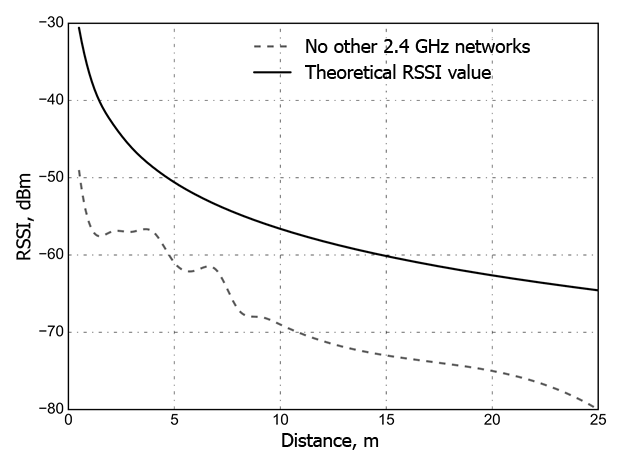
\includegraphics[clip, width=0.49\textwidth]{ch-3/fig-4a}%
		\label{ch-3/fig-4a}
	}
	\subfloat []{%
		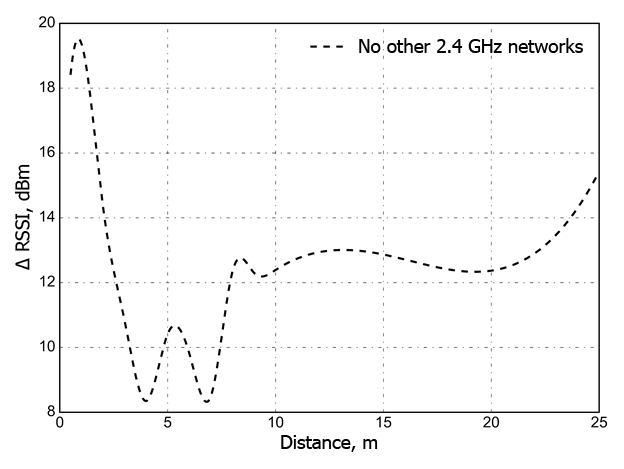
\includegraphics[clip, width=0.49\textwidth]{ch-3/fig-4b}%
		\label{ch-3/fig-4b}
	}
	\caption[Влияние характеристик приемника и передатчика на $RSSI$ и отклонение $RSSI$ от теоретического значения]{Влияние характеристик приемника и передатчика на: $RSSI$ (\textit{а}) и отклонение $RSSI$ от теоретического значения (\textit{б})}
\end{figure}

Одной из отличительных характеристик промышленного производства является тип среды, по которой распространяется беспроводной сигнал. Производство чаще всего характеризуется отражающей средой, за некоторыми исключениями, например, целлюлозно-бумажные и деревообрабатывающие предприятия, где преобладает поглощающая среда. Распространение сигнала в отражающей среде подвержено эффекту многолучевого распространения~\cite{7433518}. В результате принимаются не только прямые, но и отраженные лучи, что приводит к колебаниям амплитуды, фазы и угла входного сигнала. На рисунке~\cref{ch-3/fig-5} показаны графики $RSSI$ и $\Delta RSSI$ в зависимости от расстояния соответственно. Графики показывают значительные колебания, вызванные указанным выше эффектом.

\begin{figure} [tb]
	\subfloat []{%
		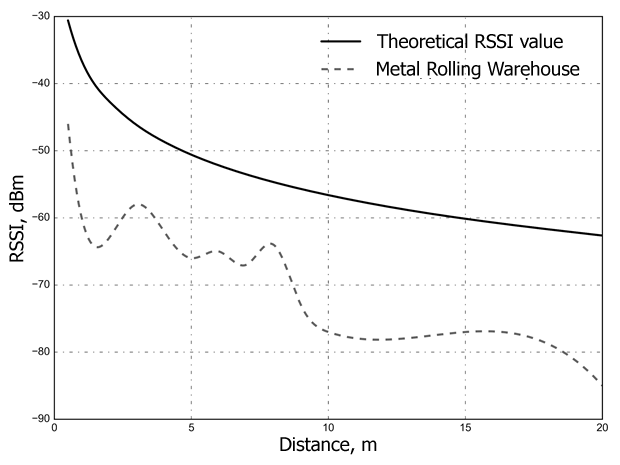
\includegraphics[clip, width=0.49\textwidth]{ch-3/fig-5a}%
		\label{ch-3/fig-5a}
	}
	\subfloat []{%
		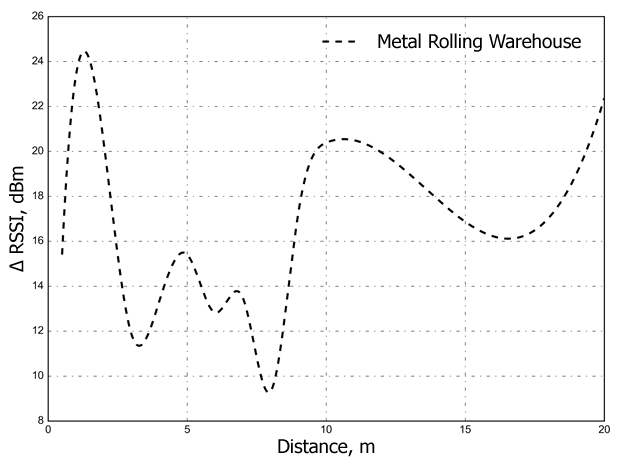
\includegraphics[clip, width=0.49\textwidth]{ch-3/fig-5b}%
		\label{ch-3/fig-5b}
	}
	\caption[Влияние отражающей среды на: $RSSI$ и отклонение $RSSI$ от теоретического значения]{Влияние отражающей среды на: $RSSI$(\textit{а}) и отклонение $RSSI$ от теоретического значения (\textit{б})}
	\label{ch-3/fig-5}
\end{figure}

Препятствия, встречающиеся на пути распространения сигнала, имеют аналогичный эффект. Кроме того, могут возникать явления дифракции (на поверхностях с резкими неровностями) и рассеяния (на шероховатых поверхностях). Стены между цехами и производственными ячейками могут отражать сигнал из-за наличия арматуры и, с другой стороны, поглощать его из-за звукоизоляции. Более того, в производственных помещениях бывают ситуации, когда приемник или передатчик может располагаться только за определенным препятствием или внутри бокса. \cref{ch-3/fig-6} показывает данные для этого случая. Полученный результат аналогичен показанному на~\cref{ch-3/fig-5}; однако отклонение $RSSI$ больше, поскольку препятствие окружало приемник и находилось в непосредственной близости от него.

\begin{figure} [tb]
	\subfloat []{%
		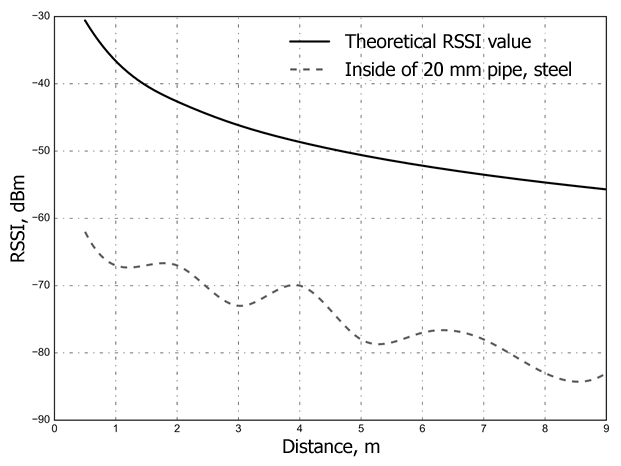
\includegraphics[clip, width=0.49\textwidth]{ch-3/fig-6a}%
		\label{ch-3/fig-6a}
	}
	\subfloat []{%
		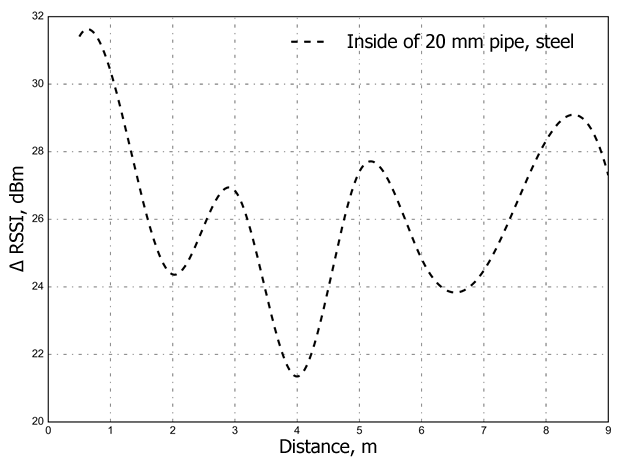
\includegraphics[clip, width=0.49\textwidth]{ch-3/fig-6b}%
		\label{ch-3/fig-6b}
	}
	\caption[Влияние препятствий в производственном помещении на: RSSI и отклонение RSSI от теоретического значения)]{Влияние препятствий в производственном помещении на: $RSSI$ (\textit{а}) и отклонение RSSI от теоретического значения (\textit{б})}
	\label{ch-3/fig-6}
\end{figure}

Поскольку инфраструктура производственной сети отличается неоднородностью, вполне вероятно, что несколько беспроводных сетей будут работать одновременно в одном и том же диапазоне частот. В этом случае может возникать интерференция и накладываться когерентные волны, что приводит к увеличению или уменьшению результирующей амплитуды. Этот эффект может быть особенно заметен, когда устройства работают на одном канале, что типично для диапазона~\SI{2,4}{\giga \hertz}, где сети Wi-Fi, Bluetooth, ZigBee и Thread пересекаются~\cite{016461}. Полученные графики в~\cref{ch-3/fig-7} показывают значительное влияние этого фактора.

\begin{figure} [htb]
	\subfloat []{%
	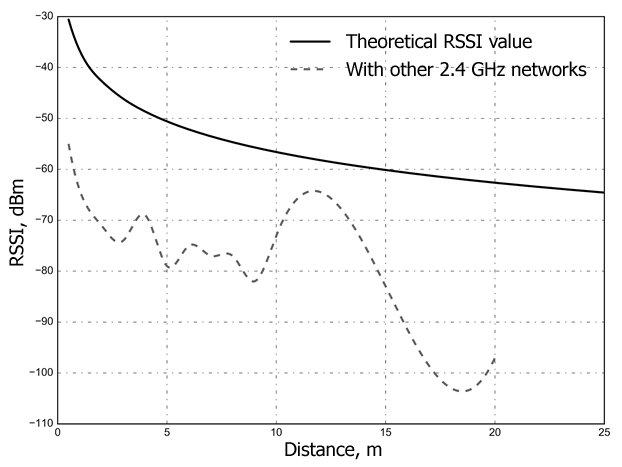
\includegraphics[clip, width=0.49\textwidth]{ch-3/fig-7a}%
	\label{ch-3/fig-7a}
	}
	\subfloat []{%
	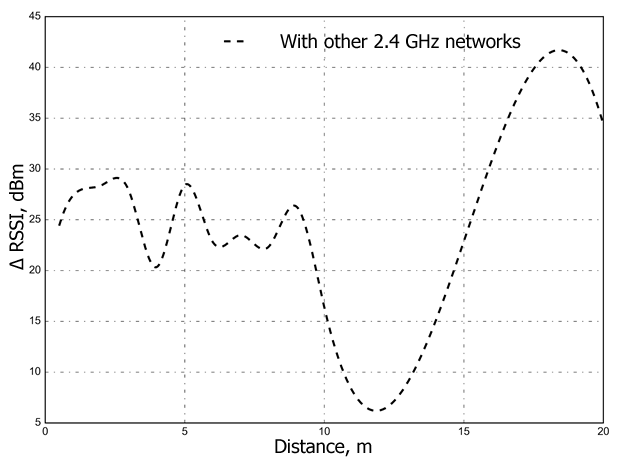
\includegraphics[clip, width=0.49\textwidth]{ch-3/fig-7b}%
	\label{ch-3/fig-7b}
	}
	\caption[Влияние соседних сетей~\SI{2,4}{\giga \hertz} на: отклонение RSSI и $RSSI$ от теоретического значения]
	{Влияние соседних сетей~\SI{2,4}{\giga \hertz} на: отклонение RSSI (\textit{а}) и $RSSI$ от теоретического значения (\textit{б})}
	\label{ch-3/fig-7}
\end{figure}

Большое количество силового оборудования, расположенного в помещении цеха, может искажать передаваемый беспроводной сигнал и вызывать помехи. Чаще всего это наблюдается при распространении импульсного сигнала по линиям электропередачи оборудования. Это происходит потому, что при формировании фронта амплитуда сигнала изменяется с большой скоростью, что приводит к появлению большого количества высокочастотных гармоник в спектре сигнала. В случае рассматриваемого в эксперименте шагового двигателя управление осуществляется с помощью широтно-импульсной модуляции (ШИМ). Графики на рисунке~\cref{ch-3/fig-8} показывают искажение беспроводного сигнала. Для асинхронного двигателя (рисунок~\cref{ch-3/fig-9}) сильных колебаний не наблюдалось, так как управление производилось без использования преобразователя частоты. Сварочный аппарат показал один из худших показателей (рисунокк~\cref{ch-3/fig-10}), так как при переключении транзисторных ключей инвертора в процессе сварки на фронтах импульсов происходит большое количество кратковременных переходных процессов в виде затухающих высокочастотных колебания.\footnote{Электронный ресурс: {\tiny\url{https://303421.selcdn.ru/soel-upload/clouds/1/iblock/e03/e036d5c6f8c271c7ebbf44799619f068/201002052.pdf}} (дата обращения 01.05.2020).}

\begin{figure} [htb]
	\subfloat []{%
	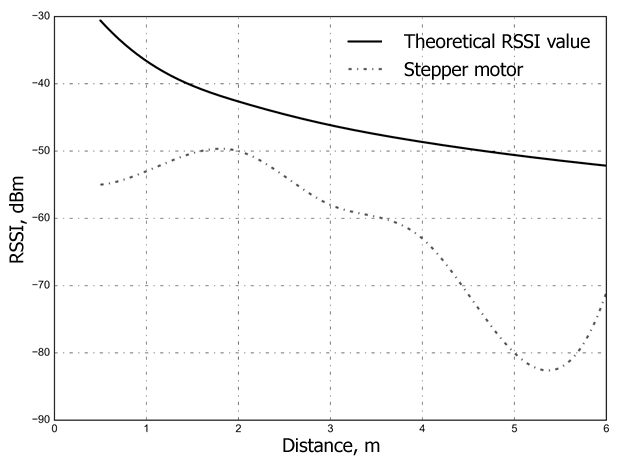
\includegraphics[clip, width=0.49\textwidth]{ch-3/fig-8a}%
	\label{ch-3/fig-8a}
	}
	\subfloat []{%
	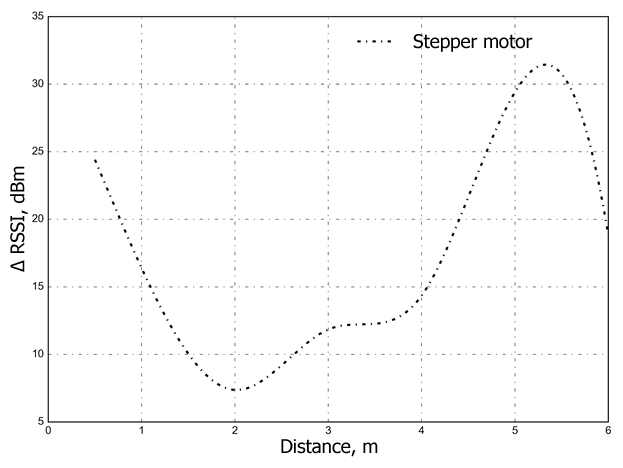
\includegraphics[clip, width=0.49\textwidth]{ch-3/fig-8b}%
	\label{ch-3/fig-8b}
	}
	\caption[Влияние исправного шагового двигателя на: отклонение $RSSI$ и $RSSI$ от теоретического значения]
	{Влияние исправного шагового двигателя на: отклонение $RSSI$ (\textit{а}) и $RSSI$ от теоретического значения (\textit{б})}
	\label{ch-3/fig-8}
\end{figure}

\begin{figure} [htb]
	\subfloat []{%
	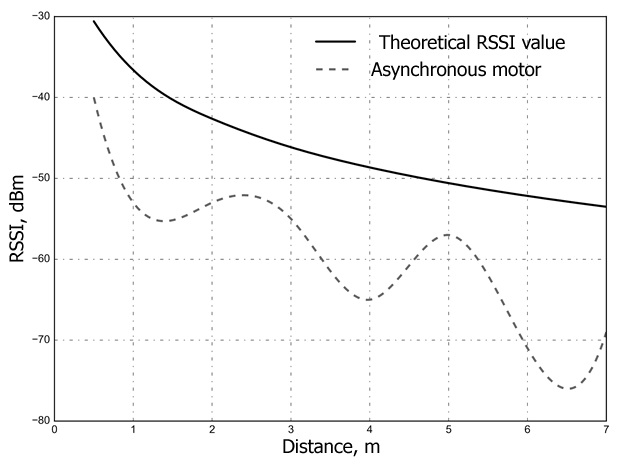
\includegraphics[clip, width=0.49\textwidth]{ch-3/fig-9a}%
	\label{ch-3/fig-9a}
	}
	\subfloat []{%
	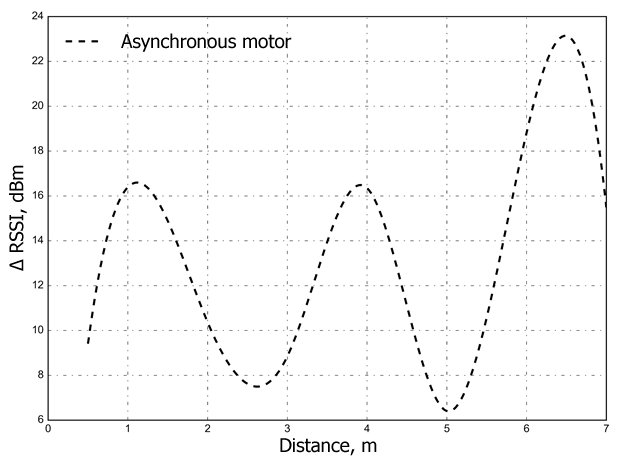
\includegraphics[clip, width=0.49\textwidth]{ch-3/fig-9b}%
	\label{ch-3/fig-9b}
	}
	\caption[Влияние работающего асинхронного двигателя на: отклонение $RSSI$ и $RSSI$ от теоретического значения]
	{Влияние работающего асинхронного двигателя на: отклонение $RSSI$ (\textit{а}) и $RSSI$ от теоретического значения (\textit{б})}
	\label{ch-3/fig-9}
\end{figure}

\begin{figure} [htb]
	\subfloat []{%
	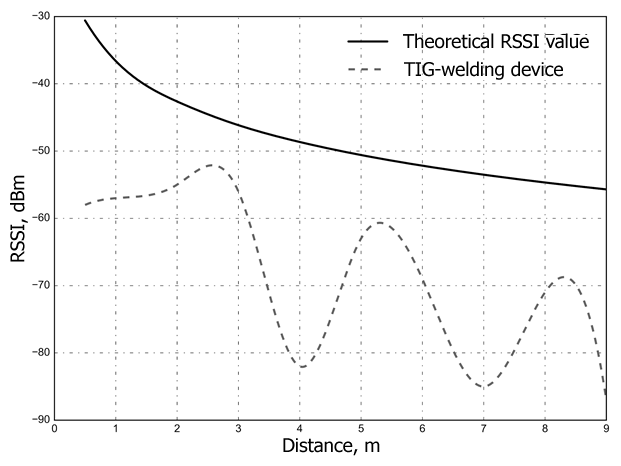
\includegraphics[clip, width=0.49\textwidth]{ch-3/fig-10a}%
	\label{ch-3/fig-10a}
	}
	\subfloat []{%
	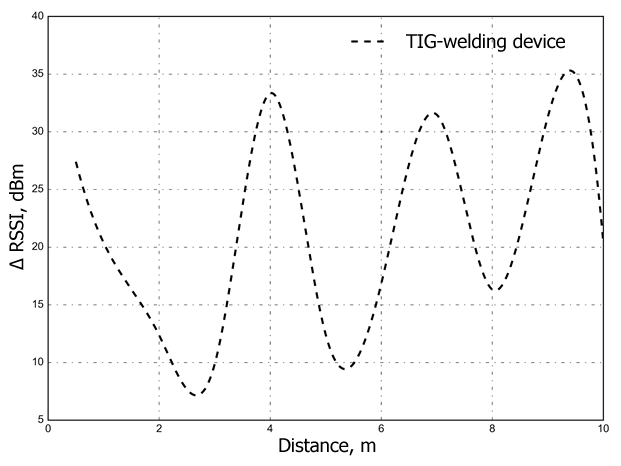
\includegraphics[clip, width=0.49\textwidth]{ch-3/fig-10b}%
	\label{ch-3/fig-10b}
	}
	\caption[Влияние работающего сварочного аппарата на: отклонение $RSSI$ и $RSSI$ от теоретического значения]
	{Влияние работающего сварочного аппарата на: отклонение $RSSI$ (\textit{а}) и $RSSI$ от теоретического значения (\textit{б})}
	\label{ch-3/fig-10}
\end{figure}

В таблице~\cref{tab-2} приводятся результаты серии экспериментов. Наихудший результат был получен в эксперименте, когда приёмник был помещен в толстостенную стальную трубу. Это означает, что такого размещения приемника следует избегать или его следует располагать не дальше~6,85\,м от передатчика. Наилучшие результаты были показаны при измерении RSSI в свободной среде.

\noindent Имеется небольшое отклонение от теоретического значения. Из-за некоторых аппаратных особенностей антенны, которые не учитывались в расчетах, и среднего теоретического значения показателя затухания. В заключении необходимо отметить, что возможность организации WPAN на основе топологии ячеистой сети позволяет нейтрализовать негативные эффекты за счет плотного расположения сетевых узлов, согласно рассчитанному~$D_{max}$.

\begin{table}[!htb]
\centering
\caption{Влияние производственных факторов на помехозащищенность беспроводных персональных сетей (WPAN)} \vspace{4pt}
\label{tab-2}
\begin{threeparttable}
\begin{tabularx}{\linewidth}{@{} lrrr}
	\toprule
	\textbf{Факторы} &
	{\small $\Delta R$} \tnote{1} &
	{\small $\Delta R_{max}$} \tnote{2} &
	{\small $D_{max}$} \tnote{3} \\
	\midrule
	Свободная среда без других сетей \SI{2,4}{\giga\hertz} & 12,37 & 18,82 & 34,22 \\
	Асинхронный двигатель & 12.69 & 19.37 & 33.99 \\
	Отражающая среда (склад металла) & 16.33 & 23.39 & 22.54 \\
	Шаговый двигатель & 17.51 & 29.41 & 19.67 \\
	Сварочный аппарат & 21.11 & 34.35 & 13.01 \\
	Среда с шумом от других сетей \SI{2,4}{\giga\hertz} & 25,03 & 32,37 & 8,27 \\
	Экранирование толстостенной стальной трубой & 26,67 & 34,41 & 6,85 \\
	\bottomrule
\end{tabularx}
\begin{tablenotes} \footnotesize
	\item [1] Средняя ошибка $\Delta RSSI$, дБм
	\item [2] Максимальная ошибка $\Delta RSSI_{max}$, дБм
	\item [3] Максимальное расстояние между передатчиками, м
\end{tablenotes}
\end{threeparttable}
\end{table}

\section{Выводы по главе 3}

Данная глава посвящена исследованию методик информационного взаимодействия компонентов системы управления модульным оборудованием. В главе представлена архитектура модульной децентрализованной системы управления, в основе которой лежит распределённый реестр, содержащий все данные о составе и структуре единицы модульного оборудования, а также комплекса модульных установок, если их несколько. Каждая единица в данном случае представляется узлом иерархической базы данных в формате JSON. Отдельные параметры называются слотами, в слоты записываются конкретные параметры модулей. Каждая единица оборудовани характеризуется коммуникационными параметрами, выполняемыми функциями и возвращаемыми значениями с допустимым диапазоном для проверки. При этом в основе каждой установки находится шасси, которое в информационном плане агрегирует информацию о модулях и осуществляет первичную автоналадку всех систем. Под выполняемыми функциями модулей подразумеваются G, M и прочие коды ISO-7bit коды, которые могут быть реализованы средствами того или иного модуля. 

С технической точки зрения модули и шасси взаимодействуют по протоколу Thread. Поддерживается как проводное,так и беспроводное подключения. Thread позволяет организовать сеть ячеистой топологии с автообнаружением узлов. Данные между узлами сети передаются через безброкерную очередь сообщений NanoMsg, формат передачи данных "--- уже упомянутый JSON, упакованный в бинорный вид.  

Для определения максимальной пропускной способности ячеистой сети было произведено исследование различных прикладный программных библиотек. Было показано, что лучшее время упаковки/распаковки и степень сжатия данных JSON продемонстрировала библиотека CBOR. Было определено, что степень сжатия не зависит от объёма исходного файла JSON. По результатам анализа также был сделан вывод, что наиболее подходящий размер сообщения "--- от 1 КБ до 100 КБ. Были произведены расчёты общей производительности связки протокола NanoMsg и упаковщика CBOR. Расчеты показали, что полоса пропускания этого канала данных находится в диапазоне от \SI{6}{\percent} до \SI{95}{\percent} от средней пропускной способности сети при использовании сокетов TCP, что можно считать хорошим результатом для этого типа программного обеспечения.

Также был проведён ряд экспериментов, которые определяют помехоустойчивость беспроводного способа передачи данных в производственной среде. Предложен метод оценки помехозащищенности сетей на основе параметра $RSSI$. Выявлены факторы ослабления беспроводного сигнала и рассчитаны значения помехоустойчивости на реальной производственной площадке.

Учитывая полученные данные, можно сделать вывод, что многие производственные факторы оказывают существенное влияние на качество сигнала в беспроводной сети. Однако воздействие недостаточно велико, чтобы полностью отказываться от использования этой технологии. Более того, влияние многих факторов может быть уменьшено за счет применения топологии ячеистой сети и плотного расположения приемников и передатчиков. Стоит подчеркнуть важность проведения соответствующих измерений для каждого конкретного производства, поскольку это обеспечивает эффективное размещение приемников и передатчиков в производственных помещениях.

\FloatBarrier